\documentclass[letter,12pt]{book}

%%% My math packages
\usepackage{enumerate}
\usepackage{amsmath}
\usepackage{amssymb}
\usepackage[amssymb]{SIunits}

\usepackage{graphicx}


\usepackage{array}      % for >{\centering\arraybackslash} etc.
\usepackage[table]{xcolor}   % table option gives cell colors




%\usepackage[normalem]{ulem}

%%% ChatGPT boilerplate for 1in margins, no header-footer, 12pt sans-serif font, with title page
% Margins
%\usepackage[margin=1in]{geometry}
\usepackage[margin=1in]{geometry}

% Double spacing
\usepackage{setspace}
%\doublespacing

% Call the chapters "Lab"
 \renewcommand{\chaptername}{Lab}
%\addto\captionsenglish{\renewcommand{\chaptername}{Lab}}

% to give reliabile vspace segments allowing answers from students at a particular place in the text
\usepackage{needspace}
\newcommand{\answerspace}[1][4cm]{%
  \par\Needspace{#1}%
  \noindent\begin{minipage}[t][#1][t]{\linewidth}\end{minipage}\par
}

\usepackage{multicol}

% adjust the itemized lists
\usepackage{enumitem}
% Global tightening for all lists (itemize, enumerate, description)
\setlist{
  topsep=4pt,      % space above and below the whole list (between paragraph and list)
  partopsep=0pt,   % extra space when list starts a new paragraph
  itemsep=2pt,     % space between items
  parsep=0pt       % extra vertical space within an item that contains paragraphs
}
% define a special list called "equipment"
\newlist{equipment}{itemize}{1}
\setlist[equipment]{label=\textbullet, leftmargin=*, topsep=0pt, itemsep=1pt, parsep=0pt, partopsep=0pt}


% global control for question formatting
\newlength{\AnswerSpace}            % default size for answer space
\setlength{\AnswerSpace}{4\baselineskip} % change this to taste

%
% Question Formatting
%
% questions environment and a command \Q[<height>]{<question text>}
\newenvironment{questions}
 % {\begin{enumerate}[label=\textbf{Question \arabic*:}, leftmargin=*]}
  {\begin{enumerate}[leftmargin=*]}
  {\end{enumerate}}
% \Q[<optional-vspace>]{Question text}
% optional argument is a length (eg. 3\baselineskip, 2cm). If omitted uses \AnswerSpace.
\newcommand{\Q}[2][]{%
  \item #2\par
  \vspace{%
    \ifx\\#1\\\AnswerSpace\else#1\fi
  }%
}

% links within and to web pages
\usepackage{hyperref}
\hypersetup{
    colorlinks=true,     % false: boxed links; true: colored links
    linkcolor=red,       % color of internal links
    citecolor=blue,      % color of links to bibliography
    filecolor=blue,      % color of file links
    urlcolor=blue        % color of external links
}

% San-serif font
\renewcommand{\familydefault}{\sfdefault}
\usepackage{sfmath}
\renewcommand{\familydefault}{\sfdefault}

% DEFINITIONS should use this ``defterm'' macro, and  will generally be bold-font, but could be changed universally here
% (I will use regular itemize without bullets for all definitions)
\newcommand{\defterm}[1]{\textbf{#1}}




%%%%%%%%%%%%%%%%%%%%%%%%%%%%%%%%%%%%%%%%%%%%%
%                               Getting subtitles on Chapters (from chatGPT)
%%%%%%%%%%%%%%%%%%%%%%%%%%%%%%%%%%%%%%%%%%%%%
\usepackage{titlesec}

% Global toggle to show/hide subtitles
\newif\ifshowsubtitles
\showsubtitlestrue     % show subtitles by default
% \showsubtitlesfalse  % uncomment to hide them

% store the current chapter subtitle here
\newcommand{\labsubtitletext}{}            % initially empty
\newcommand{\labsubtitle}[1]{\gdef\labsubtitletext{#1}}

% chapter formatting (uses \chaptername and \thechapter)
\titleformat{\chapter}[display]
  {\normalfont\huge\bfseries}              % format for whole block
  {\chaptername\ \thechapter}              % label (e.g., "Lab 1")
  {20pt}                                   % separation
  {\Huge}                                  % before-code (applied to title)
  [\vspace{1ex}\normalfont\large\itshape%
     \ifshowsubtitles\labsubtitletext\fi]  % after-code: print subtitle if enabled

% convenience command that sets subtitle, issues \chapter, then clears subtitle
\newcommand{\ChapterWithSubtitle}[2]{%
  \labsubtitle{#2}% store subtitle
  \chapter{#1}% typeset chapter (subtitle printed by titlesec after-code)
  \gdef\labsubtitletext{}% clear stored subtitle
}
%%%%%%%%%%%%%%%%%%%%%%%%%%%%%%%%%%%%%%%%%%%%%


%%%%%%%%%%%%%%%%%%%%%%%%%%%%%%%%%%%%%%%%%%%%%
%%%%%%%%%%%%%%%%%%%%%%%%%%%%%%%%%%%%%%%%%%%%%
%%%%%%%%%%%%%%%%%%%%%%%%%%%%%%%%%%%%%%%%%%%%%
\begin{document}

%%%%%%%%%%%%%%%%%  Title page  %%%%%%%%%%%%%%%%%%%%%%
\begin{titlepage}
    \centering
    \vspace*{\fill}
    {\Huge Lab Manual\par}
    {\Large The Physics of Climate Change\par}
    \vspace{1in}
    {\large Ben Holder and Tim Evans\par}
    {\large GVSU Physics\par}
    Fall 2025
    \vspace*{\fill}
\end{titlepage}
%%%%%%%%%%%%%%%%%%%%%%%%%%%%%%%%%%%%%%%%%%%%%


%%%%%%%%%%%%%%%%%  Table of Contents  %%%%%%%%%%%%%%%%%%%%%%
\tableofcontents

%%%%%%%%%%%%%%%%%%%%%%%%%%%%%%%%%%%%%%%%%%%%%
%                        Week 01  ---   Measurement and Uncertainty
%%%%%%%%%%%%%%%%%%%%%%%%%%%%%%%%%%%%%%%%%%%%%

\include{chapter_01_measurement-uncertainty-temperature}

%%%%%%%%%%%%%%%%%%%%%%%%%%%%%%%%%%%%%%%%%%%%%
%                        Week 02  ---   Global Average Temperature
%%%%%%%%%%%%%%%%%%%%%%%%%%%%%%%%%%%%%%%%%%%%%


\include{chapter_02_global-average-temperature}


%%%%%%%%%%%%%%%%%%%%%%%%%%%%%%%%%%%%%%%%%%%%%
%                        Week 03  ---   Energy and Equilibrium
%%%%%%%%%%%%%%%%%%%%%%%%%%%%%%%%%%%%%%%%%%%%%




\chapter{Energy and Equilibrium}

%%%%%%%%%%%%%%%%%%%%%%%%%%%%%%%%%%%%%%%%%%%%%
\section*{Equipment List}

\begin{multicols}{2}   % change 2 -> 3 for three columns
\begin{equipment}
  \item Ruler
  \item Stopwatch
  \item Graph paper
  \item Glass thermometer, plastic rod stirrer  (or some way of shaking?), 50mL grad cyl (2?) 
  \item Leaky Bucket Kit (pitcher, 100 mL grad cyln, 25 mL grad cyl, aquarium pump, pump  power control, two tubes, two binder clips)
  \item Track, cars, track-pulley, mass hanger, string (in the room, to be set up by students)
\end{equipment}
\end{multicols}


%%%%%%%%%%%%%%%%%%%%%%%%%%%%%%%%%%%%%%%%%%%%%
\section{Introduction and Definitions}

Today we first introduce Newton's dynamical theory of {\em motion}, for the purpose of defining {\em energy}.  We will then show that energy becomes a more general concept in physics --- beyond just the {\em kinetic energy} of moving bodies and the energy transferred from one object to another by {\em work done by a force} --- to include the thermal physics concepts of heat, internal energy, and temperature, which are of primary concern in climate science.  Specifically, it is considered a physical law of the universe that ``energy is conserved'': although it might change from one form to another, every ``drop'' of it must be acounted for... it is neither created nor destroyed.  The special case of {\em equilibrium}, where energy into a system is exactly balanced by energy out of a system, will be demonstrated using water as an analog for energy.\\[-6pt]

\noindent Note that there are a few tasks to complete within this section, \underline{highlighted with underlines}.

\subsection{Motion}

Before understanding {\em why} things move the way the do, we first must be able to {\em describe} motion.  Physicists do this by defining three related quantities for an object:
	%
	\begin{equation*}
	\text{\bf position: } x\,,  \quad\quad  \text{\bf velocity: } v = \frac{\Delta x}{\Delta t} \,, \quad \quad  \text{\bf acceleration: } a= \frac{\Delta v}{\Delta t}
	\end{equation*}
	%
We will sometimes use vector notation for these quantities, e.g., $\vec{v}$ and $\vec{a}$, to show that they point in some direction (you don't just drive 65 mph, but you drive 65 mph East). But we will calculate using the above equations and assume that the motion is just along a straight line, called the $x$ axis. In that case there are two ``directions'': in the same direction as the positive $x$ axis (positive values) and in the opposite direction (in the negative $x$ direction, negative values).  

Position is simply {where the object is} (e.g., on the $x$ axis), and velocity should be mostly intuitive --- {\em how fast is the object going} --- but also contains the direction of motion.  A nice way to understand  the relationship between velocity and acceleration is to consider the cases of ``speeding up'' and ``slowing down.'' Consider the picture below and \underline{draw the pair acceleration and velocity} \underline{{\em vectors}} (arrows) for each car, where the left car is approaching a red light and the right one has just left the intersection after the light turned green.  Label your vectors $\vec{v}$ and $\vec{a}$.
%
\begin{center}
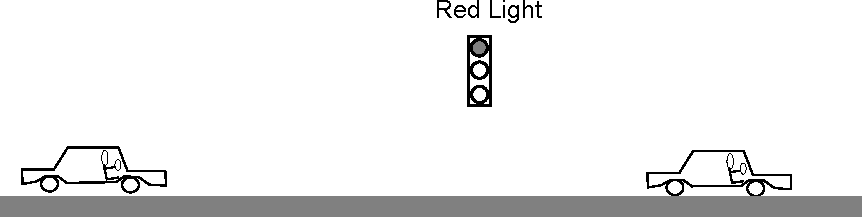
\includegraphics[width=0.8\textwidth]{images/03_red-light-speeding-slowing}
\end{center}
%
Now \underline{choose an $x$ axis} along the road by drawing an $x$-$y$ axis (your {\em choices} are: the position of the origin, and the positive $x$ direction). Then \underline{state whether each vector corresponds to a positive} \underline{or negative} one-dimensional value (you can just draw a ``($+$)'' or ``($-$)'' next to each). 

\subsection{Dynamics: Newton's Law(s)}

In 1687, Isaac Newton (English mathematician and physicist) published ``The Principia\footnote{It was written in Latin and the full title was: {\em  Philosophiæ Naturalis Principia Mathematica} (Mathematical Principles of Natural Philosophy).},'' which revolutionized human understanding of motion and its causes.  Prior to Newton, it was believed that the physical law proposed by Aristotle (Greek, 384--322 BCE) explained motion, essentially: {\em Objects move when pushed,  and stop moving when no longer pushed} \footnote{This might seem like a good law based on your own observations of the world (you're not alone: it held for 2000 years!). But it turns out that it is simply a good law for motion in a frictional fluid, like air.  If you add friction to Newton's correct description of motion, you obtain Aristotle's principle.}.  Following in the footsteps of Copernicus and Galileo, Newton proposed a better law of motion ({\bf Newton's Second Law}):
	%
	\begin{equation*}
	\textit{Objects change their motion when pushed} \quad\quad \text{or} \quad\quad \sum \vec{F} = m \vec{a} \quad \text{or} \quad\quad \vec{a} = \frac{\sum \vec{F}}{m}
	\end{equation*}
	%
where $\vec{F}$ is a {\bf force} (e.g., a push or pull interaction), the notation $\sum \vec{F}$ means ``the sum of all forces on the object'', and $m$ is the {\bf mass} of the object (e.g., in kilograms).  So Newton discovered that interaction {\em forces cause changes in velocity}.  Put another way: if there are no forces acting ($\sum \vec{F} = 0$) then there is no change to the velocity --- the object continues to move with the same velocity (vector).

Go back up to the two accelerating car(s) at the stoplight.  \underline{Draw a third vector} for each car called ``$\vec{F}$'' to indicate the force direction on the car that is causing its acceleration.  \underline{What do you think is causing} \underline{that force on the car(s)?}  (What is the {\em object} exerting the force?)

\vspace{0.5cm}

\subsection{Energy: Mechanical Energy}

The origin of the concept of energy in physics is through a quantity called {\bf Work}:
	%
	\begin{quote}
	Work is the energy transferred to an object by a force, found as {\em force times distance traveled}.
	\end{quote}
	%
or, as an equation:
	%
	\begin{equation*}
	W = F \Delta x  = \text{ Force} \times \text{distance } \quad \text{(positive when $\vec{F} \parallel \Delta \vec{x}$, negative when opposite)}
	\end{equation*}
	%
The connection of work to motion is that work causes changes in velocity.  Specifically, it changes what is called {\bf kinetic energy} of an object:
	%
	\begin{equation}
	K = \frac{1}{2} m v^2 	\quad \quad  \text{(Kinetic Energy, motional energy)}
	\end{equation}
	%
by the {\bf ``Work-Energy Theorem''}:
	%
	\begin{quote}
	The total work on an object is equal to the change in its kinetic energy: $W = \Delta K$.
	\end{quote}
	%
Another type of mechanical energy is {\bf Potential Energy}, which is stored energy (the potential to do work and cause kinetic energy). Common examples are springs (compressing an object against a spring) and gravity (raising an object up); in each case, ``releasing'' the object will allow the stored energy to be converted into motional kinetic energy.

For mechanical systems that have no friction, energy is always {\em conserved}: it can change from kinetic to potential, but will not be lost or gained.

\subsection{Energy: Other Energy}

Materials constructed from atoms (either the free-flowing fluids of liquids and gases, or the rigid lattices of solids) contain {\bf internal energy}.  If we think of these systems as just collections of little particles, then: (i)  a fluid's internal energy is determined by sum of the kinetic energy of all particles bouncing around in the container; (ii) a solid's internal energy is contained in the kinetic energy of the vibrating particles, and in the potential energy of the ``springs'' that connect them together.  When the number of particles in a material becomes very large, we treat the object as a thermal system: the {\em temperature} is a measure of the average internal energy of the particles.

There are other types of energy, some of which we will consider later: energy from electromagnetic radiation (light), electrical currents, nuclear energy.

\subsection{Energy: Equilibrium}

For an object that is both receiving enegy and giving away energy, we say that the object is in {\bf equilibrium} when:
	%
	\begin{quote}
	Rate of Energy In $=$ Rate of Energy Out  \hspace{1cm} (Equilibrium)
	\end{quote}
	

\section{Experiments and Activities}


\subsection{Motion}

Find a ``frictionless'' track and car and bring it to your lab bench.  Set it up and make sure that it is level by adjusting the ``feet.''  In each of these two experiments
	%
	\begin{enumerate}
	\item On a level track, give the car a kick at one end, and have your partner stop the car before it reaches the other end.
	\item Raise one end of the track and give the car a kick (not enough to go off the other end), then catch it.
	\end{enumerate}
	%
	perform the following tasks:
	%
	\begin{itemize}
	\item Do the experiment with the car (be sure to catch it before it reaches the ends).
	\item Time the experiment to get a range of times for your experiment.
	\item Observe the motion of the car during the whole time.
	\item Plot a position ($x$) vs time graph, and a velocity ($v$) vs time graph below it, as we did in lecture.
	\item Identify on the graph any time periods where the car is {\em accelerating}.  (How can you tell?)
	\end{itemize}
	%

\subsection{Mechanical Work}

Attach a pulley to the end of your track. Cut a long (3~m) piece of string and attach it to the car and to a mass-hanger with some amount of weight.
	%
	\begin{itemize}
	\item Record the amount of mass on your mass hanger (including the hanger itself).  Calculate the {\em weight}\footnote{The Weight of an object is the force of gravity on the object, $W = F_g = m g$, where $m$ is the mass in kilograms, $g$ is the ``acceleration due to gravity'' (10 m/$s^2$). The units on this product, kilograms times meters per second squared, are called {\em Newtons}, N.} of this amount using $\text{weight} = F_g = mg$.
	\item Do a few trials where you release the mass hanger from just below the table, letting it pull the car.
	\item Construct the position and velocity graphs again for this motion.
	\item Describe how this experiment relates to {\em work} and the {\em ``work energy theorem''}.
	\end{itemize}
	%
Return the track, the car, and the pulleys back to their places.

\subsection{Work and thermal energy}

Complete this with your whole table (4 people): one pair doing the stirring and one doing the hand-heating.
	%
	\begin{itemize}
	\item At the sink, fill up a glass beaker with cold water.  
	\item Then fill the two 50~mL graduated cylinders with the same water, to the same level (approximately 20~mL).  Record the level and the temperature.
	\item One pair will attempt to increase the temperature of the water by {\em mechanical work} (stirring with the plastic rod).
	\item The other pair will attempt to increase the temperature of the water by conduction with your hand.
	\item Conduct the experiment at least once for two minutes and record any temperature changes.
	\end{itemize}

\subsection{Equilibrium: Leaky Buckets}

Over the next few weeks in class, we will consider the energy equilibrium of the Earth, meaning the balance between the incoming energy per second from the Sun and the outgoing energy per second that the Earth emits into space.  In turns out that, while the incoming rate (energy from the sun) is approximately unchanging, the outgoing rate {\em depends on the Earth's temperature}.   As an equation, it looks like this:
	%
	\begin{equation*}
	Rate_\text{  Sun Energy In} = Rate_\text{  Earth Energy Out} \left(T_\text{Earth} \right)
	\end{equation*}
	%
where the parentheses on the right-hand side means that the rate {\em depends} on temperature.  The importance of this dependence is that in a situation of equilibrium (when the left-hand side equals the right-hand side) the result implies a single temperature: we can determine the temperature of the Earth by assuming equilibrium.

Today we will play with an analogy of this situation: a ``leaky bucket'' that is being filled by a variable-rate pitcher.  We will see if the equilibrium flow rate depends on any properties of the system (like the rate of energy into/out-of the Earth depends on its temperature).

\vspace{1cm}

\noindent Complete the following, using the data table on the next page, and eventually making a graph on graph paper of the last two columns.
	%
	\begin{itemize}
	\item Fill the pitcher of water about $3/4$ full.
	\item Raise the blue ``lab jack'' up so that the 100~mL graduated cylinder will fit underneath the pitcher spout.
	\item Place the catch tray below the spout and then connect the aquarium pump: the pump will be sitting on the table with one rubber tube (IN) going into the catch tray, and another rubber tube (OUT) going into the pitcher.  You can test that this is working by plugging in the pump and letting the water flow from the pitcher into the catch tray, and back to the pitcher through the pump.
	\item Place the 100~mL graduated cylinder (GC) in the catch tray and let the water go out of the spout into the cylinder.  Record any general observations.
	\item Now adjust the flow from the spout so that the level of the water in the GC is just a little bit above the hole (couple mL).  
	\item On the table, record the {\em baseline} level (the value on the GC of the center of the hole).
	\item In ``Approx Level'' put ``just above hole'', and record its ``Exact Level'', and then subtract off the baseline value to get the $\Delta V$ value.
	\item Now remove the GC without changing the flow.
	\item Use the 25~mL graduated cylinder and the stopwatch to time how long it takes to fill (to the 25~mL line).  Record this in your table under ``Time to 25~mL''.  It would be best to do this three times, take the average and record the average and approximate uncertainty. You can then calculate the  ``Flow Rate'' (or you can wait to do that later for all of the data you collect).
	\item In the rest of the rows of the table, choose successively larger flow rates. The ``Approx level'' could give you a target to try and find (like ``twice the $\Delta V$ as the first'', or three times, etc), but always record the exact level that you have.
	\item In the end calculate the height in cm from the $\Delta V$ column by measuring the distance on the GC itself.  
	\item On graph paper, make a plot of your data: either Flow rate vs Height, or vice-versa\footnote{When we say ``y vs x'' we mean ``vertical vs horizontal''.}.
	\end{itemize}


\newpage
%%%%%%%%%%%%%%%%     DATA TABLE         %%%%%%%%%%%%%%%%%%%%%%%%
\renewcommand{\arraystretch}{1.4}

\begin{center}
\begin{tabular}{|p{2.5cm}|p{2.5cm}|p{2.5cm}|p{2.5cm}|p{2.5cm}|p{2.5cm}|}
\hline
\textbf{Approx level} &
\textbf{Exact Level} &
\textbf{$\Delta V$}\newline (above hole) &
\textbf{Time to \newline25 mL} &
\textbf{Flow Rate} &
\textbf{Height} \\
\hline
 (  \hspace{1cm} )  & (  \hspace{1cm} )  &(  \hspace{1cm} ) & (  \hspace{1cm} ) & (  \hspace{1cm} )  & (  \hspace{1cm} )  \\   % units row
\hline
\hline
Baseline Value (Hole Center) &  &  \cellcolor{gray!90}  &  \cellcolor{gray!90} &  \cellcolor{gray!90}   &  \cellcolor{gray!90}  \\[1.5em]
\hline
 & & & & & \\[1.5em]
\hline
 & & & & & \\[1.5em]
\hline
 & & & & & \\[1.5em]
\hline
 & & & & & \\[1.5em]
\hline
 & & & & & \\[1.5em]
\hline
 & & & & & \\[1.5em]
\hline
 & & & & & \\[1.5em]
\hline
 & & & & & \\[1.5em]
\hline
 & & & & & \\[1.5em]
\hline
\end{tabular}
\end{center}
Be sure to fill in the units in the second row.








 

%%%%%%%%%%%%%%%%%%%%%%%%%%%%%%%%%%%%%%%%%%%%%
%                        Week 04  ---   Electromagnetic Specrum and BB Radiation
%%%%%%%%%%%%%%%%%%%%%%%%%%%%%%%%%%%%%%%%%%%%%


\ChapterWithSubtitle{Electromagnetic Radiation and Blackbody Radiation}{All the light you cannot see}

%%%%%%%%%%%%%%%%%%%%%%%%%%%%%%%%%%%%%%%%%%%%%
\section*{Equipment List}

\begin{multicols}{2}   % change 2 -> 3 for three columns
\begin{equipment}
  \item IR camera (w/ cable)
  \item NIR security camera (w/ cable)
  \item ``go-pro'' camera (w/ cable)
 % \item UV lights
 \item NIR LED light panel
 \item wooden block (``stage'')
 \item bathtoy (``character'')
 \item 250 mL beaker
  \item cardboard box
  \item large (12in square) plastic window
  \item small (3in square) plastic window
  \item small plastic window, blacked out
  \item TV remote
  \item Silicon disks
  \item Coke or Diet Coke or Coke Zero
  \item Faraday Cage with radio
\end{equipment}
\end{multicols}

\noindent {\bf Note:} Today will will make observations of light with a few different cameras.  You will submit on Blackboard the usual pdf of the lab assignment and your written work, but then you can just submit extra images (jpg files) in addition the pdf ({\bf do not print images or add them to your pdf}). If you need to correct a submitted pdf, just submit another one; I will only use the last pdf document.  Image files can be obtained from the IR thermal camera by plugging it into the computer with the USB-C to USB cable; it will appear as a drive with a DCIM directory.  Images from the ``go-pro/active'' visual light camera and the near-IR ``security'' webcam can simply be screenshotted or downloaded using the Camera app on the windows PC.  {\bf Every student should get their own copies of the relevant images} and save them to their email or to, e.g., drive.google.com.  

%%%%%%%%%%%%%%%%%%%%%%%%%%%%%%%%%%%%%%%%%%%%%
\section{Introduction and Definitions}

Today we consider light, in all of its colors/wavelengths.  The collection of light of all wavelengths is called the {\bf electromagnetic spectrum} (because light, it turns out is a propagating wave of electric and magnetic fields). Objects with a nonzero absolute temperature (having any internal energy) will {\bf radiate} light of a wavelength/color that is specific to their temperature.  The idealization of this is called {\bf blackbody radiation}, because perfect emitters are also perfect absorbers (``black''). 

\subsection{Electromagnetic Spectrum}

Light is an oscillating {\bf electromagnetic wave} with a characteristic wavelength, which we usually write as the greek letter ``lambda,'' $\lambda$.  The range of wavelengths that we are able to see with our eyes is called {\bf visible} light and spans a range of wavelengths from \unit{0.40}{\micro\meter} (blueish light, \unit{400}{\nano\meter}) to \unit{0.75}{\micro\meter} (reddish light, \unit{750}{\nano\meter}).

Consider the schematic wave below and the red blood cell given for scale.  Sketch two waves, one that has the wavelength of red light, and one that has the wavelength of blue light, making them to scale with the blood cell image.
%
\begin{center}
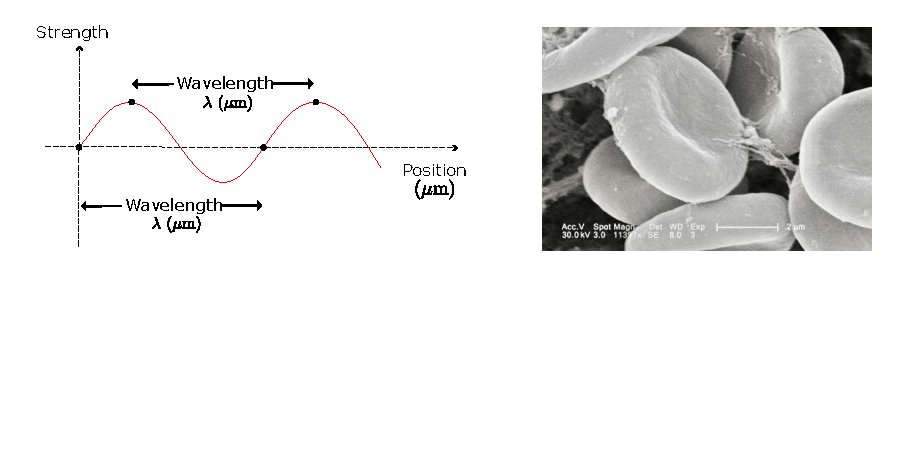
\includegraphics[width=0.9\textwidth]{images/04_scale-wavelength-rbc.pdf}
\end{center}
%
Now consider the rest of the electromagnetic spectrum.  We give the names to ranges of wavelength values: gamma-rays, X-rays, ultraviolet, visible, near-infrared, infrared/far-infrared, microwave, radio.   
	%
	\begin{itemize}
	\item Look up the wavelength ranges of these types of light and \underline{make a table}, putting all wavelengths in micrometer ($\mu$m).
	\item On the wavelength axis below (in log scale) show the range of each type of light.  [Notice that $\unit{10^0}{\micro\meter} = \unit{1}{\micro\meter}$ (and $10^{1} =10$, $10^{-1} = 1/10$), and that the midpoint between $1$ and $10$ on a logarithmic scale is 3.]
	\end{itemize}
	%
	%
\begin{center}
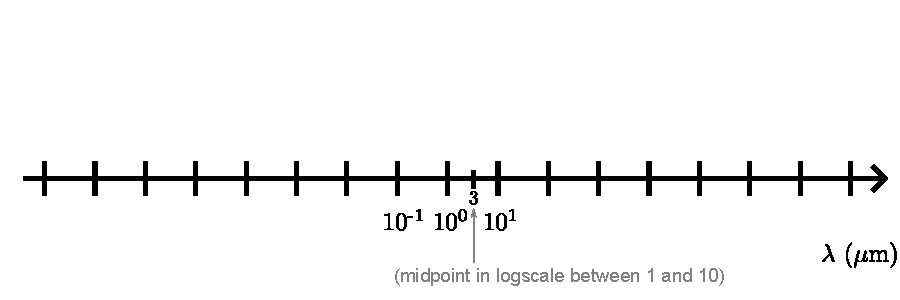
\includegraphics[width=0.9\textwidth]{images/04_EM-spectrum-logscale}
\end{center}

\subsection{Blackbody Radiation}

Any object that has internal energy will have a temperature greater than absolute zero ($\unit{0}{\kelvin} = -273\degree$C); and it turns out that any object with a temperature radiates light.    This phenomena is called {\bf blackbody radiation}.   There are a few key equations that describe the amount and wavelength of light emitted by blackbody radiators:
%
\begin{equation*}
\lambda_\text{peak} = \frac{\unit{2900}{\micro\meter \cdot \kelvin}}{T} \quad \quad \text{Wien's Law, wavelength of peak emission}
\end{equation*}
%
\begin{equation*}
F = \left( 6 \times 10^{-8} \, \frac{\text{J}/\text{s}}{\text{m}^2 \cdot \text{K}^4}\right) T^4 \quad \quad \text{Stefan-Boltzmann Law (total flux)}
\end{equation*}
%
\begin{equation*}
F_\lambda = \frac{F}{1.5 \times \lambda_\text{peak}} \quad \quad \text{Peak value of ``Spectral Flux''}
\end{equation*}
%
Our Sun is the most familiar example of a (nearly) ideal blackbody radiator.  It has a temperature of about \unit{6000}{\kelvin}.  What is the wavelength of the peak of its blackbody radiation?  What is its total flux?

\vspace{3cm}

A table is given below showing the spectral emission or sensitivities of equipment we will use in the lab today.  Fill in the last column with the temperatures corresponding to blackbody radiators with peaks at the wavelengths given (one temperature if a single value, two temperatures if a range is given). There is space for calculation examples below.
%
\begin{center}
\begin{tabular}{|l|l|l|}
\hline
Device & Wavelength range ($\mu$m) \hspace{1cm} & BB Temperatures \hspace{2cm} \\
\hline
\hline
% WRONG IN F2025???   
%Mileseey IR Camera & \unit{4.6}{\micro\meter} -- \unit{11.5}{\micro\meter} & \\
Mileseey IR Camera & \unit{8}{\micro\meter} -- \unit{14}{\micro\meter} & \\
\hline
ELP USB NIR (webcam) & \unit{0.4}{\micro\meter} -- \unit{1.0}{\micro\meter} & \\
\hline
ELP USB NIR (illuminators) & \unit{0.94}{\micro\meter} & \\
\hline
Andoer IR49S LED Panel & \unit{0.855}{\micro\meter} & \\
\hline
Andoer IR49S LED Panel & \unit{0.855}{\micro\meter} & \\
\hline
AKASO v50 elite action camera & \unit{0.40}{\micro\meter}  -- \unit{0.70}{\micro\meter} & \\
\hline
\end{tabular}
\end{center}
%

\vspace{4cm}


\section{Experiments and Activities}


\subsection{Observations of light}

We have equipment for observing light in the (far) infrared (the Mileseey camera); in the near infrared (NIR) (the ELP webcam); and the visual range (your eyes and the AKASO ``action camera'').  For the NIR (and comparisons between NIR and visual) you can put the cameras and objects under the cardboard box to get a dark environment.  Objects with a temperature (at your table, around the room) can serve as sources of infrared light.  The Andoer LED panel acts as a source of near IR light.

\vspace{0.25cm}

\noindent For each item of observation, \underline{make and document (with words and images) some observations}.  Some things to try, and questions to answer:
	%
	\begin{itemize}
	\item Use the infrared camera to observe objects and people (with their permission!) around the room.  
	\item Try to see the ``ghosts'' of warm objects when they are removed from another object (your hand on the table or wall).
	\item Spill a bit of water on the floor and see what it looks like.
	\item See if various lights change in the IR picture when on/off.
	\item What are warm objects and cold objects in the room \ldots anything surprising?  (Note the temperature output on the image itself).
	\item Place the security camera and the visual camera under the box with a ``stage'' (little block) and a ``performer'' (bath toy animal).  How do their view compare?
	\item Put the NIR LED panel in the box as well, and document the visual and NIR camera views.
	\item Can you see the NIR LEDs with your eye?  
	\item Can anything see the bulb in the TV remote when you press its buttons?
	\item How does the NIR webcam see things?  Is it the same idea as the IR camera?  How do such ``security cameras'' work, and why are they designed this way?
	\end{itemize}

\subsection{Observations of transmission of light}

Whether an object is called {\bf transparent} or {\bf opaque} turns out to be wavelength dependent.  What does this mean in plain language?

\vspace{5cm}

\noindent Now make some observations.  Some things to try and questions to answer:
	%
	\begin{itemize}
	\item Use the ``clear'' plastic window, with various sources and cameras.
	\item Use the silicon plates (be careful they are fragile, but you can put your fingers on them) with various sources and cameras.
	\item Try the glass in the doorway.
	\item Fill a small beaker with coke. Place an object (pencil?) in it and observe with your eyes, the action camera, and under the box with the NIR camera and/or the visible light camera, with and without the NIR LED panel.
	\item Try out the ``faraday cage'' and the AM/FM radio.  Two local stations are WGVU (88.5 MHz) and WOOD (1300 KHz).  What are the wavelengths of these broadcast stations (calculate using $c = \lambda f$, where the speed of light is $c = \unit{3 \times 10^8}{\meter/\second}$).
	\item Does the faraday cage affect cell-phone signals?
	\end{itemize}






 

%%%%%%%%%%%%%%%%%%%%%%%%%%%%%%%%%%%%%%%%%%%%%
%                        Week 05  ---   Heating by Radiation, Specific Heat
%%%%%%%%%%%%%%%%%%%%%%%%%%%%%%%%%%%%%%%%%%%%%



\ChapterWithSubtitle{Heating by Radiation}{Feel sun on your face. No one else can feel it for you.}
%\chapter{Heating by Radiation}

%%%%%%%%%%%%%%%%%%%%%%%%%%%%%%%%%%%%%%%%%%%%%
\section*{Equipment List}

\begin{multicols}{2}   % change 2 -> 3 for three columns
\begin{equipment}
\item Calorimetry kit: Calorimetry can, aluminum cylinder, 250~mL beaker
\item Heating by Radiation kit: aluminum block, styrofoam holder with kickstand, no-slip pad, large mass
\item Digital thermometer
\item 100~mL graduated cylinder
\item styrofoam cups (for getting ice)
\item incandescent desk lamp
\item graph paper
\item cooler of ice (for room)
\item scale (for room)
\item active camera (optional)
\item computer (optional)
\end{equipment}
\end{multicols}

%\noindent {\bf Note:} Today

%%%%%%%%%%%%%%%%%%%%%%%%%%%%%%%%%%%%%%%%%%%%%
\section{Introduction and Definitions}

To estimate the energy balance of the Earth, and thus estimate its expected equilibrium temperature, we must first know the input energy to Earth system: the radiation flux (in $\frac{\text{J}/\text{s}}{\text{m}^2}$) from the Sun.  Recall our ``leaky bucket'' experiment: When you increased the flow of water coming out of the pitcher, you observed a rising water level in the graduated cylinder (the leaky bucket), until the point at which the rate of water spraying out of the hole match the incoming rate of flow from the pitcher.  When that equilibrium was achived, there was an equilibrium height of the water above the hole\footnote{That height determines the rate of flow out of hole, essentially by conservation of mechanical energy: a larger column of water in gravity, leads to a larger kinetic energy of the exiting water.}.  We can make an exact analogy to the energy balance of the earth: the Sun pours energy into the Earth through photons of light; the Earth sprays energy back into space because it has a temperature (specifying its internal energy) and therefore radiates as a a blackbody; and when these two rates of flux are equal, the internal energy of the Earth stops changing, leading to an ``equilibrium level'' of temperature.  Today we would like to directly measure the amount of energy being ``poured in'' by the Sun.  (Or, if the Sun does not cooperate, an incandescent light bulb).

\subsection{First Law of Thermodynamics, Heating, and Calorimetry}

In our introduction to the topic of energy --- beginning with the work by a force, generalized to include all types energy transfer mechanisms, and all types of internal and external energy types --- we emphasized the basic physical law: energy is conserved\footnote{Although it may change its form, and transfer from one object to another, the total amount of energy never changes.}.  Most generally, energy conservation is stated as a law within thermodynamics (the physical topic of heat, temperature, and chemistry) and is given the grand title {\bf The First Law of Thermodynamics} (FLTD):
	%
	\begin{equation*}
	\Delta E_\text{tot}  = Q + W \,.
	\end{equation*}
	%
This equation pertains to any single object/system that you choose and summarizes the rules we used in the construction of energy flow diagrams: a change in the total energy of an object, $\Delta E_\text{tot}$, must be exactly accounted for by the energy input to or output from that object (on the right hand side), in the form of {\bf heat flow}, $Q$, or mechanical {\bf work}, $W$ (these flows, $Q$ and $W$, are positive when energy is coming into the system, and negative when energy is going out).

Today we will consider a special case of the above equation, where our system consists of two objects brought together at different temperatures.  There will be no work done on the system and we will consider the combined system of two objects to be ``closed'' so that there is no heat flow in or out of the system.  In that case, we have:
	%
	\begin{equation*}
	\Delta E_\text{tot}  = Q + W  \quad \rightarrow \quad \Delta E_\text{tot} = 0 + 0 \quad \rightarrow \quad \Delta E_1 + \Delta E_2 = 0\, ,
	\end{equation*}
	%
which says that the sum of the internal energy changes in the two sub-objects must equal zero.  Another way to view the combined system is to break it into two objects.  In that case we would have two equations (one equation for each ``object'' box, in an energy flow diagram):
	%
	\begin{equation*}
	\begin{array}{c}
	\Delta E_{\text{tot}, 1}  = Q_1 + W_1 \\
	\Delta E_{\text{tot}, 2}  = Q_2 + W_2 \\
	\end{array} 
	\quad \rightarrow \quad
	\begin{array}{c}
	\Delta E_{\text{tot}, 1}  = Q_1 + 0 \\
	\Delta E_{\text{tot}, 2}  = Q_2 + 0 \\
	\end{array} 
	\quad \rightarrow \quad
	Q_1 + Q_2 = 0
	\end{equation*}
	%
where the last equation follows from the previous two, plus our prior equation for the combined system (that the sum of the two energy changes is zero).  When drawing an energy flow diagram, there is a single transfer arrow between the two objects, which we could label with $|Q|$.  In the equation for one object, that transfer is accounted as a positive or negative value depending on whether the flow is into or out of  that object.

\underline{Consider an example system}: cold milk poured into a mug of hot coffee. We will ignore the energy loss out of the system as a whole during the time of mixing, so the above equation holds.  Sketch an energy flow diagram for these two objects during the time they are mixing (not yet at equilibrium).  

\answerspace[2cm]

Then write down three FLTD equations, like those above: one for the combined system and one each for the objects in your diagram.  Instead of ``1'' and ``2'' labels, use ``C'' and ``M''. 

\answerspace[2.5cm]

We express heat flow into an object through an equation that demonstrates its change in the internal energy of that object (essentially The {\bf heat capacity} of an object, $C$,  is the constant of proportionality between the heat transfer to/from the object and its internal energy change, as measured by a change in temperature:
	%
	\begin{equation*}
	Q = C \, \Delta T \, .
	\end{equation*}
	%
This is not a very useful equation because the value of $C$ depends on all of the details of the object.  A more fundamental quantity is the {\bf specific heat capacity} (often called simply the ``specific heat'') {\em of a material}, denoted by the lower-case $c$.  This is the heat capacity per mass of an object, so we can write:
	%
	\begin{equation*}
	Q = c \, m \, \Delta T \, .
	\end{equation*}
	%
One of the materials with the largest specific heat capacity is water, with $c_W = \unit{4.2}{ \joule/g/K}$.  This means that it takes \unit{4.2}{\joule} of energy to raise one gram of water one degree Kelvin (which, since $\Delta T_K = \Delta T_{\degree C}$, is the same amount to raise by one degree Celsius). The term ``capacity'' is used because, once you have added energy to raise the temperature, that energy is essentially stored in the water and can be transferred somewhere else.  Other materials that have a lower specific heat capacity, like aluminum,  experience a higher temperature increase for the same, $\unit{4.2}{\joule}$, energy input --- or, put another way, raising the temperature of aluminum by one degree stores less energy than raising the same amount of water by one degree (aluminum's capacity to store energy is less than water).

\underline{Write down} a $Q_1 + Q_2 = 0$ equation for the ``milk plus coffee'' example above. Again, use ``C'' and ``M'' as labels. Then use the above equations containing specific heat to express heat as a temperature difference.  The final temperature within the two $\Delta T$'s will be the same, $T_f$, but the initial temperatures will be different.  Re-write your equation to show this in variables.  Then discuss briefly why the two terms will add to zero, knowing what you do about the initial and final temperatures of the coffee and milk.

\newpage

\section{Experiments and Activities}


\subsection{Specific heat of aluminum}

Before looking at the heating of an aluminum block under the radiation of the sun (or incandescent bulb), we will first determine the specific heat capacity of the material itself.  Our experiment will be a very simple calorimetry example: prepare a small aluminum cylinder at a known temperature (letting it equilibrate with ice water) and then drop it into a vat of water while monitoring the temperature of the water.  The drop in water temperature at that instant can be associated to a heat transfer from water to aluminum, which causes an internal energy increase (decrease) of the cylinder (water). Knowing the specific heat water (and the masses of both the water and aluminum), we can determine the specific heat of aluminum.  

\noindent {\bf Procedure}: Using your own paper to write down observations, keep a data table, and make calculations from equations --- take the following basic steps.
	%
	\begin{itemize}
	\item Open up the ``calorimetry can'' and inspect it.  What are the components of it, and what is the purpose of each?  (The small cup inside is what you will fill with water).
	\item Get some ice from the cooler. Create an ice-water bath in your 250~mL beaker and place the aluminum cylinder inside.
	\item Get hot water from the faucet ($\sim50\degree$C) and fill the small calorimetry cup up to about \unit{2}{\centi\meter} (we will measure this amount after the experiment is over).
	\item Place the cup inside the calorimetry can, insert the thermometer through the ``cork'' and observe the temperature.  
	\item Start your stopwatch.
	\item When your thermometer has stopped changing dramatically (when it has come to the temperature of the water), start taking data.  These should be time and temperature measurements at approximately 30 second intervals\footnote{If you would like, you could use the go-pro-like camera to record the stopwatch and thermometer --- probably best to record with the ``time-lapse'' feature --- and then get (temperature, time) data points by watching the video afterwards.  Think carefully about how to do this ahead of time.}. It is probably easiest to simply record the time on the stopwatch (4m50s) and then later you can convert  that (in an additional column) to the number of seconds (290~s). Create a table of your temperature vs.\ time data.  
	\item While you are still getting temperature measurements on the water use a second thermometer, to check that the ice water and cylinder mixture is at the right temperature.  You can stir it up to make sure it is reaching equilibrium.
	\item Once you have taken about five minutes of data of the water alone, use the tongs to grab the cylinder and drop it into the warm water (be sure you're not carrying any ice with you).
	\item Record the time that the cylinder was added, but let the stopwatch keep running.
	\item Continue to measure the temperature at stopwatch times for another 5 minutes, again at  approximately 30 second intervals.
	\item Make a graph of temperature vs.\ time on graph paper.  Be sure to choose axes such that your data covers most of the page.
	\item Using a ruler, make two best-fit straight lines, before and after the time at which the cylinder was inserted.
	\item At the time the cylinder was inserted, draw a vertical line.  The intersection of this with your two best-fit lines will give you a $\Delta T$ for the water (vertical interval length), as well as the initial and final temperature values of the water.
	\item Carefully remove the aluminum cylinder from the calorimetry can (without losing any water). Then, using the digital scale, measure and record the mass of the aluminum cylinder. 
	\item Take your small calorimetry cup to the sink, along with your 100~mL graduated cylinder.  Pour the water into the graduated cylinder to record the volume of water in the can.  (Think ahead of time about how to do this since your water volume will likely be more than 100~mL!)  The conversion from volume to mass is the density equation, $\rho = m / V$, where the density of water has the very nice value, $\rho_W = \unit{1.0}{\gram/\milli\liter}$.
	\item Sketch an energy flow diagram, for the water and cylinder objects, showing the heat flow and energy changes in the time immediately after placing the aluminum cylinder in hot water, but before they reach equilibrium.
	\item Then write down equations to arrive at a $Q_\text{Al} + Q_\text{W} = 0$ equation, like you did in the introduction. Use this final equation to calculate the specific heat capacity of aluminum. Recall that the specific heat capacity of water is $c_W = \unit{4.2}{\joule/\gram/\;\degree C}$.
	\end{itemize}


\subsection{ Heating aluminum block by radiation}

Now that we know the specific heat of aluminum, we can measure precisely how incoming radiation flux causes a temperature increase.  In this experiment the heating of an aluminum block will be accomplished by light (from the sun or your incandescent desk lamp) rather than conduction from a hot to a cold object. But the input heat for aluminum can be interpreted with exactly the same equation:
	%
	\begin{equation*}
	Q_\text{Al} = m_\text{Al} \, c_\text{Al} \, \Delta T
	\end{equation*}
	%
\noindent {\bf Procedure:} Using your own paper to write down observations, keep a data table, and make calculations from equations --- take the following basic steps.
	%
	\begin{itemize}
	\item Place your aluminum block into the insulating styrofoam.  If there is no hole through the styrofoam for the thermometer, measure the position of the hole in the block and carefully figure out where to pierce the styrofoam such that the thermometer will hit the hole and fit snugly into the aluminum block.
	\item Prop up the styrofoam at an angle, using its kickstand, the no-slip pad, and a large (e.g., 1~kg) mass.
	\item Arrange the desk lamp so that it is pointing at the block and quite close ($\sim \unit{5}{\centi\meter}$). Tilting the lamp to its side first, before pointing the bulb at the block, can get a better coverage. Record the distance from bulb to block.
	\item Start your stopwatch.
	\item Turn on your desk lamp.
	\item Record (time, Temperature) values in a table, every 30 seconds (or even every minute should be fine) for about 20 minutes.  Like the previous experiment, it is probably easiest to simply record the stopwatch time (and later convert it to a number of seconds).
	\item Make a graph of your data, Temperature vs.\ time.
	\item You should see that your data has a region in the middle where the temperature increases approximately linearly, in between time interval with a flatter change (when the block starts heating, and after it is starting to come to equilibrium temperature). Using a ruler, draw a straight line of best fit in the linear region.  
	\item Using two widely-separated {\em points on the line} calculate the slope of that line.
	\item This slope, $\frac{\Delta T}{\Delta t}$, can be converted into a $\frac{\Delta E}{\Delta t}$ using the specific heat capacity of Aluminum.  Write this out as an equation and then calculate the value.
	\item The power increase you just calculated can be translated into a flux, by dividing by the area of the aluminum block. Write out an equation for this, and then calculate a value.
	\item Using your distance to the lamp, you can now try to estimate the power of the light bulb.  This is the same procedure we did in class to go from the Sun's power, to its flux at the position of the Earth's orbit, but backwards.
	\end{itemize}






 

%%%%%%%%%%%%%%%%%%%%%%%%%%%%%%%%%%%%%%%%%%%%%
%                        Week 06  ---   Greenhouse (cooling block, food coloring water)
%%%%%%%%%%%%%%%%%%%%%%%%%%%%%%%%%%%%%%%%%%%%%



\ChapterWithSubtitle{Greenhouse Effect: Light Absorption and Transmission}{There's a light.}
%\chapter{Heating by Radiation}

%%%%%%%%%%%%%%%%%%%%%%%%%%%%%%%%%%%%%%%%%%%%%
\section*{Equipment List}

\begin{multicols}{2}   % change 2 -> 3 for three columns
\begin{equipment}
\item Coin
\item Ruler
\item Stopwatch
\item Aluminum block 
\item Foam holder without kickstand
\item Scissors 
\item Aquarium (no lego top necessary)
\item Food coloring set
\item Ulanzi (multiple-color-mode LED light)
\item Desk lamp
\item Blue Tape
\item Digital Thermometer
\item Apron
\item 250 mL beaker
\item Stirring stick 
\item computer
\item Bin of 14cm x 20cm mylar sheets (shared)
\item Graph paper (shared)
\item Gloves  (shared)
\end{equipment}
\end{multicols}




%\noindent {\bf Note:} Today

%%%%%%%%%%%%%%%%%%%%%%%%%%%%%%%%%%%%%%%%%%%%%
\section{Introduction and Definitions}

Today we will start investigating how light interacts with matter.   In the past few weeks, we calculated the Earth's equilibrium temperature\footnote{See our discussions for the past two weeks, and Chapter 4 in our textbook by Dessler.} by assuming that it was in energy equilibrium: the incoming average flux from the Sun was exactly balanced by the outgoing (blackbody, infrared) flux of the Earth.  When we assumed an Earth without an atmosphere, we found that the equilibrium temperature would be about -18$\degree$C (0$\degree$F). But when we assumed that there was atmosphere --- i.e., a greenhouse gas atmosphere: blocking all of the Earth's infrared light, and then re-radiating as an infrared blackbody, according to its own temperature --- then we found that the equilibrium temperature of Earth's surface rises to about +30$\degree$C (86$\degree$F). Although both of these estimates are incorrect --- the actual average surface temperature\footnote{In the coming weeks we will account for energy flow through water vapor and derive a more accurate estimate.} of the Earth surface is about 15$\degree$C --- the presence of the atmosphere and its so-called {\em greenhouse effect} are incredibly important to make a livable environment.

To understand the greenhouse effect, we must understand why and how the Earth's radiation is captured by the atmosphere. More specifically: why and how is infrared light is captured by molecules of greenhouse gases [e.g., water vapor ($\text{H}_2\text{O}$), carbon dioxide ($\text{CO}_2$), and methane ($\text{CH}_4$)].  To answer the ``why'' we will investigate, in lecture and discussion, the mechanism by which light (electromagnetic waves) interacts with the electric dipole (overall neutral, but a slight separation of positive and negative charges) of these molecules.  Interaction with infrared light in particular (as opposed to visible, ultraviolet, and other bands) causes vibration and rotation of these molecules\footnote{Intractions with shorter wavelength light generally causes things like excitation of the electrons in the atoms, or ionization (removal) of these electrons.}. Essentially, greenhouse gases are those that have an electric dipole which can be ``grabbed'' by the light to induce such effects, while non-greenhouse gases [like oxygen ($\text{O}_2$) and nitrogen ($\text{N}_2$)] have no electric dipole, and thus no interaction with the light.  Although this explanation comes from the classical theory of electricity and magnetism, the actual interaction is {\em quantum}.  Light is a quanta (photon, packet) of electromagnetic radiation with fixed energy (determined by its wavelength: $E = h c / \lambda$). A photon's encounter with a molecule is a random process in which capture occurs some {\em probability}.  Absorption causes the ``excitation'' of the molecule, meaning that it will begin to oscillate or rotate. And then the excited molecule lose its excitation by randomly emitting a photon with the same energy (at a random time and in a random direction).\\[-6pt]

\noindent \underline{Make a sketch for yourself below of this interaction process} in a sequence of three pictures side by side.  In the first (left), draw the light photon as a little ``bump'' with sinusoidal waves inside it, approaching (show a velocity vector) a molecule (e.g., $\text{H}_2\text{O}$ is a big O ball connected by rods to two small H balls).  In the second (center) the photon has been absorbed but now the molecule rotates or vibrates. And in the third (right), the molecule has shot the photon off in a random direction.

\vspace{4cm}

\subsection{The ``how'' of greenhouse gas absorption: exponential losses}

As described above, the ``why'' of light-matter interaction (the best theory physicists have to explain the process) involves a random capture of photons by molecules, which then redirects the light into a random direction.  The net effect of many such encounters --- which we might call the ``how'' of greenhouse gas absorption --- is that a beam of light (a beam of many photons) passing into a region with greenhouse gas will lose its forward progress rapidly.  Although no energy is lost --- each photon is absorbed into rotational/vibrational energy, then re-emitted in a random direction --- the number of photons that pass completely through region will drop off exponentially (literally!) with distance.  Let's perform a small experiment to see why that is the case.\\[-6pt]

\noindent \underline{Using the table on the next page} perform a coin-flip experiment.  Each row in the table corresponds to an incoming photon of light and each column at right corresponds to a layer of the atmosphere.  The first column should be the label of the photon; label them 1--20. The second column wil be the ``zeroth layer.'' Put a mark in the box for each row/photon of that second column to indicate that the photon is traveling to the right prior to any encounters. The third column is the first layer.  In this column, you will put a mark only if the photon has passed through the layer without being captured.  You will determine the fate of each photon by flipping a coin: each photon has a 50\% chance of passage.  So, flip the coin 20 times to determine whether each row in the first later gets a mark or not.  In the next column (the second layer) you will only flip a coin for the photons/rows that made it through the first layer.  And so on, until you have no more photons.  \\[-6pt]

\noindent \underline{Now make a data table} below with two columns, $(N_\text{layers}, N_\text{photons})$, showing the number of photons surviving after each layer.  On the computer, open a google sheets document\footnote{At: \texttt{sheets.google.com}} enter this data (with column headers for the titles).  Make a plot of the data using the following steps:
	%
	\begin{itemize}
	\item Highlight the two rows of data (including header names).
	\item Select {\em Insert}/{\em Chart}. And a chart will appear showing your data.
	\item On the {\em Chart Editor} at right, change the {\em Chart type} to {\em Scatter}.
	\item Make a second chart following the same previous three steps. Click on the vertical axis labels to bring up the {\em Vertical Axis} menu. Check the {\em Log Scale} check box.
	\item Now click one of the data points to bring up the {\em Data Series} menu. Check the {\em Trendline} box. Change the {\em Type} to {\em Exponential}. Then choose {\em Use Equation} under {\em Label}.
	\end{itemize}
	%
Now upload your data to the common spreadsheet for the class.  Once everyone has done so, make one more graph using the average data for the class.  Comment on what the graphs look like (in particular, how does an exponential functionlook when plotted in a ``log-linear'' fashion).  Speculate what these results mean for the Earth's light passing into the atmosphere.

\newpage

%%%%%%%%%%%%%%%%%%%%%%%%%%%%%%%%%%%%%%%%%%%%%%%%%%%%%%%%%
%                                          Table for photon absorption coin-flip experiment
%%%%%%%%%%%%%%%%%%%%%%%%%%%%%%%%%%%%%%%%%%%%%%%%%%%%%%%%%
\begin{center}
\begin{tabular}{|p{1.3cm}|p{1.3cm}|p{1.3cm}|p{1.3cm}|p{1.3cm}|p{1.3cm}|p{1.3cm}|p{1.3cm}|p{1.3cm}|p{1.3cm}|}
\hline
\textbf{Label} &
\textbf{Layer0} &
\textbf{Layer1} &
\textbf{2} &
\textbf{3} &
\textbf{4} &
\textbf{5} &
\textbf{6} &
\textbf{7} &
\textbf{8} \\
\hline
\hline
&  &   &   &    &  &   &   &    &    \\[0.8em]
\hline
&  &   &   &    &  &   &   &    &    \\[0.8em]
\hline
&  &   &   &    &  &   &   &    &    \\[0.8em]
\hline
&  &   &   &    &  &   &   &    &    \\[0.8em]
\hline
&  &   &   &    &  &   &   &    &    \\[0.8em]
\hline
&  &   &   &    &  &   &   &    &    \\[0.8em]
\hline
&  &   &   &    &  &   &   &    &    \\[0.8em]
\hline
&  &   &   &    &  &   &   &    &    \\[0.8em]
\hline
&  &   &   &    &  &   &   &    &    \\[0.8em]
\hline
&  &   &   &    &  &   &   &    &    \\[0.8em]
\hline
&  &   &   &    &  &   &   &    &    \\[0.8em]
\hline
&  &   &   &    &  &   &   &    &    \\[0.8em]
\hline
&  &   &   &    &  &   &   &    &    \\[0.8em]
\hline
&  &   &   &    &  &   &   &    &    \\[0.8em]
\hline
&  &   &   &    &  &   &   &    &    \\[0.8em]
\hline
&  &   &   &    &  &   &   &    &    \\[0.8em]
\hline
&  &   &   &    &  &   &   &    &    \\[0.8em]
\hline
&  &   &   &    &  &   &   &    &    \\[0.8em]
\hline
&  &   &   &    &  &   &   &    &    \\[0.8em]
\hline
&  &   &   &    &  &   &   &    &    \\[0.8em]
\hline
\end{tabular}
\end{center}
%%%%%%%%%%%%%%%%%%%%%%%%%%%%%%%%%%%%%%%%%%%%%%%%%%%%%%%%%
%%%%%%%%%%%%%%%%%%%%%%%%%%%%%%%%%%%%%%%%%%%%%%%%%%%%%%%%%

\newpage

\section{Experiments and Activities}


\subsection{Cooling by radiation, with blankets}

We will revisit our aluminum block from last time, but this time we will heat it up and watch it lose its heat to the environment.  You will heat the aluminum block to approximately 50$\degree$C (as you see below, we will just put it in warm water this time), then place it in its little foam holder and measure the temperature over time to estimate again $\frac{\Delta T}{\Delta t}$.  \\[-6pt]

\noindent Draw an energy flow diagram for the block below (after it has been heated and left in its holder) and say a few words about how you think the cooling takes place, i.e., what are the mechanisms of energy flow out of the block that cause its decrease in internal energy.

\vspace{6cm}

\noindent In our experiment, however, each pair of experimenters will use a different number of mylar (``shiny space blanket'') sheets to cover the block during the time it is cooling.  Draw a second energy flow diagram for this situation (it will be essentially the same as our diagram for the Earth with atmosphere, from Discussion last week, but not in equilibrium), and discuss the differences.

\vspace{6cm}

\noindent {\bf Procedure:} Using your own paper to write down observations, keep a data table, and make calculations from equations --- take the following basic steps.
	%
	\begin{itemize}
	\item Prepare a space blanket for your aluminum block by taping together one or more mylar sheets.  We will discuss with the whole class to get a variety of layer numbers among all pairs.
	\item Using tape, attach the blanket to end of the foam holder that has a hole in it. Poke your thermometer through the blanket such that it goes through the hole (and can enter the aluminum block).
	\item At the sink, run the hot water into the provided trays until they are filled with approximately 50$\degree$C water.  Drop your aluminum block inside and let it warm up for a minute.
	\item Bring your aluminum block back to its holder, cover it with its blanket. Insert the thermometer and make sure it goes into the aluminum block before taping down the blanket to the other sides.
	\item Start your stopwatch and start taking (time, temperature) data.  You might use a google sheets spreadsheet with columns for [minutes, seconds, t (s), T (C)]; that makes it easy to write down the time on the stopwatch (mm:ss) and later calculate how many seconds have elapsed for the ``t (s)'' column.
	\item Take data for 10--15 minutes, about once a minute.
	\item Remove and disassemble your space blanket, returning the individual mylar sheets to their bin.
	\item Make plot of your data using graph paper.  
	\item Using a ruler, draw a best-fit line through the data.  Calculate the slope using two widely-separated points {\em on your line of best fit}.
	\item Upload your value of $\frac{\Delta T}{\Delta t}$ to the common class google sheet, indicating the number of mylar layers used in your blanket.
	\item Later, if time permits, use google sheets to plot all of the data from the class: $\frac{\Delta T}{\Delta t}$ vs.\ $N_\text{layers}$.  
	\end{itemize}
	%


\newpage


\subsection{Transmission of light through water (with colors)}

Here we will determine how food coloring changes the amount of light that passes through water in the little aquariums provided.  You have a light source (``Ulanzi'') that can provide white light at different temperatures and intensities, as well as single-color light at diffferent intensities.  We will pass that light through the water and observe how much gets through (when clear, and with multiple drops of food coloring added), using an app on your phone called the ``Physics Toolbox Sensor Suite''.    Go to your app store now and try to install that app for at least two phones at your table.  Once you have the app, you will use the ``Light Meter'' mode. Let me know if you have trouble getting it.

\subsubsection{Calibration}

\noindent To start we will determine the sensitivity range of our phone cameras.  Fill your aquarium almost full of water. Turn off the classroom lights and give yourself some personal light with the desk lamp but not pointed toward your aquarium (you want the phone app to observe only the light from the Ulanzi). Put the light source pointing into the water at the center of one of the long sides.  You might place the light on its flat side, and elevate it above the table (on masking tape or other platform) to make sure it is flush to the side of the aquarium, while still being fully below the water. Then place your phone on the other side.    Adjust the app so that camera being used is pointing through the aquarium.   Turn on the light with the switch on the side.  Change modes by holding down (long-pressing) the button-wheel on back. Change between Intensity and Temperature/Color by short-pressing the button. Turn the wheel to change the values.  As you take data you can hold your phone in your hand to make it flush with the side as well. Move the phone around until you get the maximum Lux reading and record that.   \\[-6pt]

\noindent {\bf Procedure:}
	%
	\begin{itemize}
	\item Set your light on white light (long press to get to that mode), but at a lower temperature than then Sun (so maybe around $\sim$3000 K). Turn up the Intensity.  (Single pressing the button takes you between Intensity and Temperature.)
	\item Place your phone in position so that it is observing through the aquarium and is giving a ``Lux'' value.
	\item In a new Google Sheets document, make a table with (Intensity, Lux) columns.  Intensity is the thing shown on the light itself (between 0 and 100) and Lux is what is read off the phone app.
	\item Turn down the Intensity of the light and record a new value.  Repeat this procedure multiple times so that you can see how your phone observes different intensities.  What you should find is that there is a large range of intensities where the phone camera is saturated\footnote{On my old iPhone, saturation happens between 20\% and 100\% for the ``5800 K'' light, but on newer phones, the camera is saturated all the way down to 2\% Intensity!  With a ``3000 K'' light you should be able to find an unsaturated range below 20\%.}, meaning that you always get the same, maximum, Lux value.  Take a few data points in this range and then turn down the Intensity such that the Lux values start changing, and take more (5--6) data points in that range.
	\item Using Google Sheets, make a graph of this data (Lux vs.\ Intensity).  You should find that there is a saturation value for your phone, but that for Lux values well below that, it is approximately linear.  
	\item Write down the max ``Lux'' setting that you can trust (this should be a value below the curve starts to saturate.
	\end{itemize}


\subsubsection{Experiment} %
Now we will consider how the light passing through the aquarium changes as you put more and more drops of food coloring into it.  At your table of four, each pair should choose a different color (use Blue or Red).  You can test your dropper skills in a 250~mL beaker of water before dropping into the aquarium.  There are aprons and gloves available to protect you from food coloring drops.  Set the initial light brightness (as measured by your phone) so that it is not oversaturated, as you determined in the ``Calibration'' section.\\[-6pt]

\noindent Before performing the experiment, read through the procedure.  Give a brief statement below about what you expect to see in the final graphs.\\[-6pt]

\vspace{4cm}

\noindent {\bf Procedure:}
	%
	\begin{itemize}
	\item Make a new table of ``Lux'' vs.\ number of food coloring drops.  You can do this in Google Sheets  You will have three ``Lux'' columns for the intensity observed in White, Red, and Blue light.  
	\item Before putting any drops in, choose an intensity for your light (checking to see that the measured Lux is ok) and then record the ``zero drops'' value of Lux for Red, Blue, and White light.
	\item Add one drop of food coloring to your aquarium and stir until homogeneous (practice the dropping in the beaker).  
	\item Record the Lux values for the three colors of light again.
	\item Repeat for 2, 3, 4, 6, and 8 drops.
	\item Use google sheets to make a graph of your three data sets (all on one graph: highlight the $N_\text{drops}$ column together with the three Lux columns).
	\item Change your vertical axis scale to logarithmic, and get the exponential fit line and its equation displayed.
	\end{itemize}
	%
\noindent Returning to your predictions before the procedure, comment on whether you were correct.  What did you see, and what does it mean?















 

%%%%%%%%%%%%%%%%%%%%%%%%%%%%%%%%%%%%%%%%%%%%%
%                        Week 07  ---   Phase Transitions I (boiling water)
%%%%%%%%%%%%%%%%%%%%%%%%%%%%%%%%%%%%%%%%%%%%%



\ChapterWithSubtitle{Evaporation of water by boiling}{water water every where}
%\chapter{Heating by Radiation}

%%%%%%%%%%%%%%%%%%%%%%%%%%%%%%%%%%%%%%%%%%%%%
\section*{Equipment List}

\begin{multicols}{2}   % change 2 -> 3 for three columns
\begin{equipment}
\item Ruler
\item Stopwatch
\item Digital Thermometer
\item Apron
\item 250 mL beaker
\item mini scale
\item hot plate
\item tongs
\item safety goggles
\end{equipment}
\end{multicols}


%%%%%%%%%%%%%%%%%%%%%%%%%%%%%%%%%%%%%%%%%%%%%
\section{Introduction and Definitions}

Today we begin a serious study of water.  Water is of course directly important to life on Earth --- it played a key role in the evolution of life from microscopic organisms to the zoo that currently populates the planet (including ourselves!), and our bodies are more than half water by weight --- but it is also a key factor in controlling the Earth's climate.  Over the past week we showed that water ($\text{H}_2\text{O}$) is an asymmetric molecule with a permanent electric dipole moment and, more importantly, it has a {\em changing} dipole moment when vibrating or rotating.  We discussed the implications of this for the greenhouse effect.  Sketch  a 3D picture of the water molecule (recall that it is {\em tetrahedral} if you include the ``lone pairs'' on the oxygen atom) and discuss very briefly the implications of its shape and its electric dipole moment on our climate.

\answerspace

\noindent This week and next we will discuss a second important way that water influences our climate --- and contributes to the full answer of the question that drives the first half of this course: {\em What is the expected equilibrium temperature\footnote{Recall our prior calculations: (i) the balance of the Sun's incoming radiation flux with the Earth's outgoing infrared radiation, $F_\text{sun} = F_\text{earth} (T)$, led to an equilibrium temperature of about $-15\degree$C; (ii) assuming an atmosphere that blocks all infrared light from the Earth's surface (and then re-emits it both out to space and back down to the surface) we found an equilibrium temperature of about $+30\degree$C. Neither of these is yet correct, since our average surface temperature is about $+15\degree$C.} of the Earth?}  The mechanism of this influence is essentially the same one that our body uses to cool us when exercising: {\em perspiration}.  Say a few words about how perspiration works for the human body --- and maybe also note some conditions that prevent it from working, or decrease its efficacy --- and try to make an energy flow diagram demonstrating why the internal energy of a body decreases during perspiration.

\answerspace[3cm]

\noindent Check in with your neighbors and instructor regarding the answers to the questions in this section.

%%%%%%%%%%%%%%%%%%%%%%%%%%%%%%%%%%%%%%%%%%%%%
\subsection{Phase transitions and water}

On one of the following pages you will find what is called a {\bf phase diagram} for water.  A fixed volume/amount of water under various temperature and pressure conditions will take different forms: solid, liquid, or gas/vapor.  Note that the ``pressure'' axis has a logarithmic scale to show a wide range of values.  Let's explore this diagram a little bit. First, from your own personal experience, describe these three phases of water very briefly.

\answerspace[2cm]

\noindent Temperature should be familiar to you. Remind yourself and your neighbors what a few familiar values in Fahrenheit correspond to in the Celsius and Kelvin scales.

\answerspace[2cm]

\noindent Pressure might be less intuitively familiar.  You may have personally experienced pressure when diving to the bottom of a swimming pool. If you're not familiar with the effect, find someone in your group who has experienced it, and ask them to describe how it felt.  This experience is due to an {\em increase} in pressure --- on top of the normal {\bf atmospheric pressure} value of our surrounding air\footnote{Atmospheric pressure is also the value of the water pressure at its surface.} ---  due to the {\em weight of water} above you.  Now, knowing that the pressure {\em outside} of our atmosphere is zero (space is a ``vacuum''), and making an analogy to the swimming pool, describe why there is a non-zero atmospheric pressure at the surface of the Earth.

\answerspace

\noindent Look up the value of our atmospheric pressure (pressure is force per area, and the standard unit is the {\em Pascal}, with  $\unit{1}{\pascal} = \unit{1}{\newton/\meter^2}$).  Also look up how much its value varies over a few days (pressure is a standard parameter reported with the weather).  State these values below and then show the approximate atmospheric pressure value on the phase diagram using a ruler to make a horizontal line across the whole figure.

\answerspace[2cm]

\noindent Now consider the process of water {\bf freezing}.  Along the line of atmospheric pressure, draw a point {\bf A} that sits in the liquid water section.  Note its temperature, $T_A$.  Then draw an arrow along the line of atmospheric pressure toward solid water.  Which direction are you going (in temperature) and at which temperature --- call it $T_f$, the temperature of freezing --- does the phase change from liquid to solid?  Also: how much would your answer for $T_f$  have changed if the atmospheric pressure line was different (e.g., ten times bigger or smaller).

\answerspace[3cm]

\noindent Today we will focus on the process of {\bf vaporization} (or, {\em evaporation}, or {\em boiling}). Go back to your $T_A$ point and draw an arrow toward vapor.  Which direction are you going (in temperature) and at which temperature --- call it $T_v$, the temperature of vaporization --- does the phase change from liquid to vapor?  

\answerspace[1.2cm]

\noindent How much would your answer for $T_v$  have changed if the atmospheric pressure line was different (e.g., ten times bigger or smaller)?  Is this the same or different than what you found for the liquid-solid transition?



%%%%%%%%%%%%%%%%%%%%%%%%%%%%%%%%%%%%%%%%%%%%%
%%%%%%%%%%%%         Phase diagram for water         %%%%%%%%%%%%%%%
%%%%%%%%%%%%%%%%%%%%%%%%%%%%%%%%%%%%%%%%%%%%%
\newpage

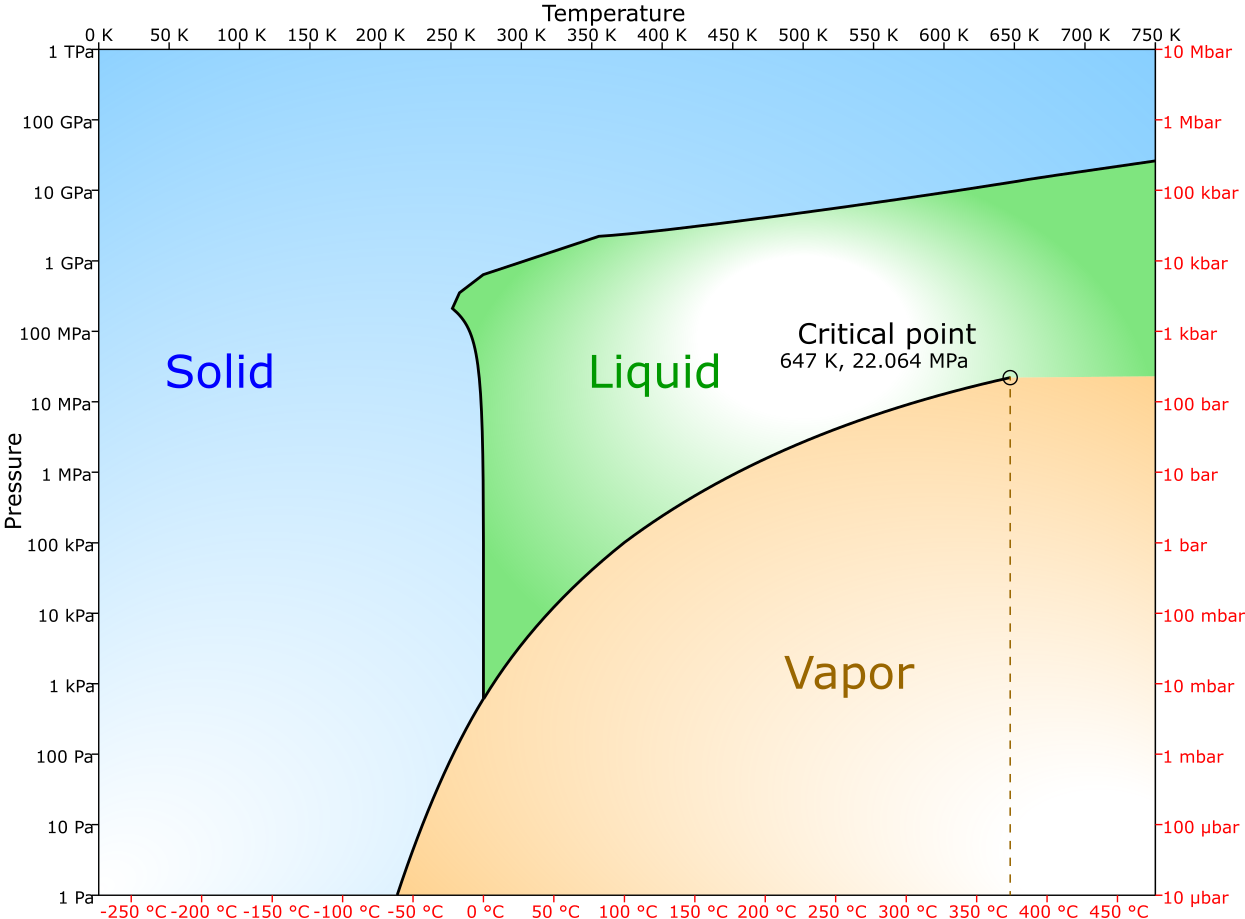
\includegraphics[width=\textheight, angle=90]{images/07_phase-diagram-of-water-simplified_wikimedia-Cmglee_edited.png}


\newpage
%%%%%%%%%%%%%%%%%%%%%%%%%%%%%%%%%%%%%%%%%%%%%
%%%%%%%%%%%%%%%%%%%%%%%%%%%%%%%%%%%%%%%%%%%%%


%%%%%%%%%%%%%%%%%%%%%%%%%%%%%%%%%%%%%%%%%%%%%
\section{Experiments and Analysis}

{\bf \underline{Safety Note}:} We will boil water on the hotplate today, and will will repeatedly transfer it back and forth from the hotplate to the scale to measure mass. You should take great care in this procedure, i.e.,  focus on tightly grasping the tongs around the beaker, just below the rim, during each transfer. Do not get distracted by other tasks or your partners while doing so. As noted in the prcedure below, it is recommended that you alternate your temperature and mass measurements so that you don't try to do two things at once.  You should also be wearing long pants and closed shoes so that if boiling water were to spill you would be partially protected. But everyone should be alert and aware during the boiling procedure as well.  You will wear safety googles for the boiling procedure to protect your eyes (these can be worn over glasses).

\subsection{Boiling water!}

We will take data on the process of vaporization using a hotplate and about 200~mL of water in a 250~mL beaker.  Our goal is to monitor both temperature and mass over time and then use the rates (of temperature increase before the ``boiling point'', and mass decrease after) to determine the so-called latent heat of vaporization, $L_v$.

\vspace{0.5cm}

\noindent {\bf Read through the entire procedure before beginning.  Listen to tips on safety and effectiveness from your instructor.}

\vspace{0.5cm}



\noindent {\bf Procedure:} Using your own paper (and/or a Google sheets spreadsheet) to write down observations, keep a data table, and make calculations from equations --- take the following basic steps.
	%
	\begin{itemize}
	\item I would recommend a google sheets spreadsheet with these columns: [minutes, seconds, t~(s), Mtot (g) , T(C)].  Then in the first two columns you can just record the time on your stopwatch (e.g., 3:53 is 3 in the minutes and 53 in the seconds column).  Later you will calculate the ``t(s)'' column values using an excel formula like ``\verb|=b2*60 + c2|''. 
	\item Place your empty beaker together with your digital thermometer on the mini scale and measure their mass together.  Record this value so that you can subtract it off from your mass measurements in the end.
	\item Put about 200~mL of tap water in your beaker.  With the thermometer inside, place it on your scale to get an initial mass measurement (your mass measurements will always include the beaker and thermometer).
	\item Start your stopwatch.
	\item Turn on your hotplate to $450\degree$C and place your 250~mL beaker of water (with thermometer) on its center.
	\item Use the blue labjack to arrange your miniscale so that it is immediately to the side of your hotplate and at the same level, so that transfers back and forth will be easier.
	\item Start taking data of temperature and mass, at approximately 1 minute intervals for each. I would recommend alternating every thirty seconds between mass and temperature, so that you don't have to take the temperature while measuring the mass.  It is perfectly fine for the temperature and mass values to be recorded at different times.
	\item For mass measurements, carefully grip the beaker with the tongs and carry it over to the scale.  Relase it and have a partner record the mass measurement.  Then grip it tightly again and bring it back to the hotplate.  This should take about 10 seconds out of every minute of warming.  Always be careful, but don't remove the beaker from the hot plate for very long.
	\item For temperature measurements, raise the thermometer above the bottom of the beaker and use it to stir for a few seconds before recording a measurement.
	\item Take data until the temperature reaches the boiling point, and then continue for at least 10 more minutes afterwards.
	\item When the experiment is finished, turn off the hotplate and move the beaker onto the table to cool. 
	\end{itemize}
	%
	

\noindent {\bf Analysis (1st Try)}
	%
	\begin{itemize}
	\item In your data spreadsheet, create a time column in seconds, as described above. Also create a new $m_w$ column by subtracting off the beaker plus thermometer mass from all of your $M_\text{tot}$ values.
	\item Create two new sheets within your google sheets document for Mass and Temperature. Transfer your mass and temperature measurements to their own sheets (highlight the data cells, choose {\em Edit} / {\em Copy}, and then use {\em Edit} / {\em Paste Special} / {\em Values}).  Within each of these  new sheets, delete any rows that do not contain that type of measurement.
	\item Make a graph of $m$ vs.\ $t$ on your Mass sheet;  and a graph of $T$ vs.\ $t$ on your Temperature sheet.  (Recall: Highlight two columns; {\em Insert} / {\em Graph}; choose the {\em Scatter} type).
	\item Look at your temperature graph and choose an interval of time prior to the boiling point\footnote{There will not be any interval where the graph is exactly linear, but linearity can be approximated over any short time.  Just avoid the early times when the hotplate was still heating up to its fixed temperature.}.    Note the values of the average temperature and average mass during that time interval (an eyeball estimate is fine).
	\item In your Temperature sheet, copy the $(t, T)$ values in your chosen time interval into two new columns. Make a chart using these new columns to get another $T$ vs.\ $t$ graph with only your selected data\footnote{This process is necessary because (i) Google Sheets doesn't allow you to do a trendline to only part of the plotted data, and (ii) Google Sheets doesn't allow you to put a second series on the same chart.}.  Click a datapoint in the graph to bring up the {\em Series} menu.  Select a {\em trendline} and change the {\em Label} to show the fitted equation.  Write down its slope as $\frac{\Delta T}{\Delta t}$.
	\item On the Mass sheet, choose an interval of time from your $m$ vs.\ t graph after the boiling point was reached. Like you did in the previous step, copy only that data to new columns and make a new graph with a trendline.  Record the absolute value of the slope as $\left| \frac{\Delta m}{\Delta t}\right|$.
	\item Follow these steps to write down two equations that express energy conservation, one during a time interval before  the boiling point and one during a time interval after the boiling point.
		%
		\begin{enumerate}[label=(\roman*)]
		\item {\bf Conservation of energy prior to boiling:} Recall from Lab 5 (``Heating by radiation'') that heating causes temperature changes in this way
			%
			\begin{equation*}
			\Delta E_\text{input} = m_w c_w \, \Delta T
			\end{equation*}
			%
		where $\Delta E_\text{input}$ is the (unknown) amount of heat energy from the hot plate into the water over a certain interval of time, $\Delta t$.  Recall also from Lab 5 that $c_\text{w}$ is the {\em specific heat capacity} of water, which we will assume to be that of pure water: \unit{4.2}{\joule/\gram/\kelvin}.  To use the slope from our temperature graph, we divide this equation by $\Delta t$ to obtain:
			%
			\begin{equation*}
			\frac{\Delta E_\text{input}}{\Delta t} = m_w c_w \, \frac{\Delta T}{\Delta t}\quad \rightarrow \quad P_\text{hotplate, before} = m_w c_w \,  \left(\frac{\Delta T}{\Delta t} \right)
			\end{equation*}
			%
		where the energy per time provided by the hotplate can be called its ``power'' input.
		
		\item {\bf Conservation of energy after boiling} After full boiling starts, you should have observed that the temperature is almost exactly constant at $100\degree$C. Therefore, no energy being used to raise the temperature of water, since $\Delta T_\text{w} = 0$, and the term with heat capacity will not appear in our equation. Instead, the heat transferred from the hot plate causes only the transition of water from liquid to vapor. This is accounted for by our {\bf latent heat of vaporization equation}
			%
			\begin{equation*}
			\Delta E_\text{input} = \left| \Delta m \right| \, L_v  \quad \rightarrow \quad \frac{\Delta E_\text{input}}{\Delta t} = \frac{\left| \Delta m \right| }{\Delta t}  \, L_v \quad \rightarrow \quad P_\text{hotplate, after} = \left|  \frac{\Delta m }{\Delta t} \right|  \, L_v 
			\end{equation*}
			%
		The first equation states that the energy input from the hotplate in some time interval, $\Delta t$,  causes a mass loss $|\Delta m|$ of liquid water into vapor (the absolute values are because the {\em change} in liquid mass is actually negative).  By dividing that equation by the time interval we have obtained an expression containing our mass graph slope, $\left| \frac{\Delta m}{\Delta t} \right|$.  
		\end{enumerate}
		%
	\item We now assume that the energy input to the water from the hotplate during the period before boiling is the same as the energy input after boiling. Therefore we can write:
		%
		\begin{equation*}
		\begin{split}
		P_\text{hotplate, before} &= P_\text{hotplate, after} \\
		m_w \, c_w \, \left( \frac{\Delta T}{\Delta t} \right) &= \left| \frac{ \Delta m }{\Delta t}  \right| \, L_v 
		\end{split}
		\end{equation*}
		%
	Solve this equation for $L_v$ and then plug in all of the numerical values you have collected.
	\item The correct value for the latent heat of vaporization of water is $L_v=\unit{2265}{\joule / \gram}$.  How did you do?
	\end{itemize}




\noindent {\bf Analysis (2nd Try)}: You might have noticed that the mass of water is decreasing slightly {\em prior to boiling}.  This means that some of the energy from the hotplate is going into vaporizing water before the boiling point.  Therefore our first equation in the prior analysis is wrong.  If we estimate the mass loss prior to boiling and account for it, we can get a better estimate of the latent heat value.
	%
	\begin{itemize} 
	\item Using your mass graph, and methods simliar to those described above, obtain a $\left| \frac{\Delta m}{\Delta t} \right|$ value for the same time interval you used to obtain $\frac{\Delta T}{\Delta t}$.  We can call this $\left| \frac{\Delta m}{\Delta t} \right|_\text{before}$.
	\item Write down a new version of the first equation, starting from:
		%
		\begin{equation*}
		\Delta E_\text{input} = m_w c_w \, \Delta T + \left| \Delta m \right|_\text{before} \, L_v
		\end{equation*}
		%
	This says that the energy input from the hotplate goes into {\em both} heating the water and vaporizing some water. Divide by $\Delta t$ to get a new power equation for ``before''.
	\item Do the same analysis as before, equating power before and after, and solve again for the latent heat of vaporization.  Notice that you have two $L_v$ variables this time, so you must combine and isolate them before plugging in numbers.
	\end{itemize}






 

%%%%%%%%%%%%%%%%%%%%%%%%%%%%%%%%%%%%%%%%%%%%%
%                        Week 08  ---   Phase Transitions II (evaporation and clouds)
%%%%%%%%%%%%%%%%%%%%%%%%%%%%%%%%%%%%%%%%%%%%%



\ChapterWithSubtitle{Evaporation and Clouds}{Show me my silver lining}
%\chapter{Heating by Radiation}

%%%%%%%%%%%%%%%%%%%%%%%%%%%%%%%%%%%%%%%%%%%%%
\section*{Equipment List}

\begin{multicols}{2}   % change 2 -> 3 for three columns
\begin{equipment}
\item Ruler
\item Hygrometer
\item Digital Thermometer
\item Ulanzi light / flashlight
\item 250 mL beaker (2)
\item 500 mL beaker 
\item Cloud chamber kit (cube with tube, felt, alcohol, caulk, baking tray, black vinyl, uranium rock)
\item Tall cloud jar w/ metal bowl for lid
\item Short cloud jar w/ glass bowl for lid
\item Dry ice chunk (instructor-provided)
\item Regular ice (in cooler)
\end{equipment}
\end{multicols}


%%%%%%%%%%%%%%%%%%%%%%%%%%%%%%%%%%%%%%%%%%%%%
\section{Introduction and Definitions}

\subsection{Atmospheric pressure and a warm-up experiment}

We have read that the the average atmospheric pressure at sea level on the Earth is about one kilogram force-equivalent per square centimeter of area ($\unit{2.2}{lb/\centi\meter^2} = \unit{14.2}{lb/in^2} = \unit{14.2}{psi} = \unit{101}{\kilo\pascal}$). This pressure is literally the weight of the column of air above us. Because liquid water is so much denser than air one can achieve an additional \unit{1}{atm} of pressure by submerging below just \unit{10}{\meter} of water\footnote{The pressure increase from the surface of a fluid to a depth $h$ is given by the equation $|\Delta P| = \rho g h$, where $\rho$ is the density of the fluid (\unit{1000}{\kilo\gram/\meter^3} for water) and $g \approx \unit{10}{\meter/\second^2}$ is the acceleration due to gravity.}.  Air pressure drops off exponentially with height in the atmosphere  with a {\em scale height} (distance over which it drops by a factor of $\frac{1}{\text{e}} \approx \frac{1}{3}$) of \unit{8}{\kilo\meter}, going to zero pressure --- a so-called {\em vacuum} --- in space.  The air pressure at Mount Everest base camp, 5,400~m above sea level, is about half what it is at sea level: $\sim \unit{50}{\kilo\pascal}$.\\[-6pt] 

\noindent{\bf Mini-experiment:} We do not ``feel'' the air pressure because it has the same value outside of our bodies (the air molecules beating against our skin) as it does internally (the water and blood molecules below our skin).  But there is a simple experiment we can do to observe its effects: evacuate the air in a soda can.  Together with your table of four students, put a small amount of water (less than  \unit{1}{\centi\meter} deep) into an empty soda can.  Heat this on a hot plate until the water has been rapidly boiling for a little while and, most importantly, the can is filled with water vapor\footnote{As we will ``see'' today, actual water vapor is invisible, so we only see its presence in the moments that it comes in contact with colder air and condenses into tiny liquid drops (what we call ``steam'').}.  By filling the can with pure water vapor, most of the air has been pushed out of the can.  If we could then rapidly condense the water vapor into liquid we would have an approximate vacuum inside the can (because the volume of {\em liquid water} associated to a can full of {\em water vapor} is miniscule).  Do this with your group by gently but quickly removing the can from the hotplate with tongs, and then turning it upside down and dunking it into a bowl of cold water.  Watch for any noticable effect on the can and document the experiment here.

\answerspace

\subsection{Phase transitions in air and partial pressure}

Last week in lab we boiled water in a 250~mL beaker.  We observed that, as expected for our classroom conditions at atmospheric pressure, boiling occured when the water reached 100$\degree$C.  Look back at the phase diagram for water that you marked up last week (Figure \ref{fig:07_phase-diagram-water}) and remind yourself why this was expected, i.e., following the horizontal line of $p = \unit{1}{atm}$ to the {\bf coexistence curve}  between liquid and vapor water.   You should have noticed in this experiment, however, that there was significant mass loss of liquid water prior to the ``boiling point.''  Mass of water dropped off rapidly once the water temperature reached 100$\degree$C (in some experiments at a rate of about \unit{3.5\times 10^{-2}}{\gram/\second}), but there was a measurable mass decline when the temperature was in the range 50--100$\degree$C  as well (a rate of about \unit{1.0\times 10^{-2}}{\gram/\second}). The reason for this is:
	%
	\begin{enumerate}[label=(\roman*)]
	\item The phase diagram we used last week pertains to {\em pure water}, i.e., liquid water in a closed container with only water vapor and ice.  This description applies to water in the bulk of the fluid, below its surface.  Once internal liquid water molecules reach 100$\degree$C, their intermolecular forces weaken and they are likely to separate from neighboring molecules to form water vapor instead, which then bubbles to the surface (``boiling'').
	\item Water molecules at the surface, however,  are exposed to air, so they are {\em not} in a ``pure'' liquid-vapor-water situation.  Generally air contains only some small percentage (precisely, a small {\em mole fraction}) of water vapor.  It turns out that\footnote{The physical reason for this result is due to the ideal gas law, where, as long as the densiities are quite low, all types of gas molecules treated as the identical non-interacting particles; so the liquid water at the surface only ``sees'' a low-density water-gas within the total air gas.} the same phase diagram can be used to determine the coexistence curve, but for pressure one must use the so-called {\bf partial~pressure} of water in air: 
		%
		\begin{equation*}
		e = f \times p_\text{atm} = \frac{n_{\, \text{H}_2\text{O}}}{n_{\, \text{H}_2\text{O}} + n_\text{dry air}} \times p_\text{atm}
		\end{equation*}
		%
	where $e$ is the variable\footnote{This is not the same ``e'' mentioned above in the ``scale height'' discussion; that was the exponential constant, or {\em Euler's number}, $\text{e} = 2.718\ldots$.} typically used for partial pressure, and $n$ is the variable for the number of moles, so $f$ is the {\em mole fraction of water in air}. Because the mole fraction of water in air is generally significantly less than one (on the order of 1\%), the partial pressure of water in air is significantly less than (about 1\% of) atmospheric pressure. 
	\end{enumerate}
	%
So, your boiling experiment was actually two separate experiments occuring at once: a pure-water phase transition occuring below the surface, and a liquid-to-vapor-in-air transition occurring at the surface.  Make a sketch of your boiling water beaker and point to the two different  water vapor pressures at the two different locations.  Sate the the variable names of these pressures and estimate their values roughly (using the ``1\%'' estimate given above).

\answerspace

\noindent We will do this more precisely in a moment, but quickly return to your phase diagram from last week  (Figure \ref{fig:07_phase-diagram-water}) to estimate the vaporization temperature for the water at the surface, where $e \approx 0.01 \times p_\text{atm}$.  Record this temperature value (as best you can read off that graph) here.

\answerspace[2cm]

\subsection{Relative humidity, absolute humidity, and dew point temperature}

\noindent The vaporization temperature for liquid water in contact with air is called the {\bf dew point temperature}.  Let's determine this value more carefully.  First look up the ``current conditions'' on a weather page (e.g., search for ``NWS 7-day grand rapids'') and record the current temperature, the {\bf relative humidity} (expressed as a percentage), and the dew point temperature. [Note: If it is currently raining and/or the humidity is greater than $\sim85\%$, choose a different data point within the ``3 Day History'' when the humidity was lower.]

\answerspace[2cm]

\noindent Now examine the so-called {\bf psychrometric chart} shown in Figure \ref{fig:08_psychrometric-and-phase-diagrams}.  Use your temperature (horizontal axis) and relative humidity (curved lines labeled at top) values to determine the associated {\bf absolute humidity} (vertical axis), which is expressed here as a ratio of water mass to (dry) air mass:
	%
	\begin{equation*}
	\text{AH} = \frac{m_{\, \text{H}_2\text{O}}}{m_\text{dry air}}
	\end{equation*}
	%
To determine the partial pressure of water in air, we must find the mole fraction, $f$, from this quantity.  \underline{Let's derive the relationship between $\text{AH}$ and $f$ now.}  \\[-6pt]

\noindent (i) Recall that the number of moles of a gas can be expressed as $n = m / M$ where $m$ is the actual mass of the volume of gas and $M$ is the {\bf molar mass} of the gas (determined by summing the molar masses given on a periodic table for each of its component atoms).  Find $M$ for water and for dry air. Remember that water is $\text{H}_2 \text{O}$, and air is basically 80\% nitrogen ($\text{N}_2$) and 20\% oxygen ($\text{O}_2$), so $M_\text{air} = 0.8 M_{\text{N}_2} + 0.2 M_{\text{O}_2}$. 

\answerspace[6cm]

\noindent (ii) Now write out the {\em mole ratio}
	%
	\begin{equation*}
	r = \frac{n_{\, \text{H}_2\text{O}}}{n_\text{air}} \, ,
	\end{equation*}
	%
using the $n = m/M$ equation in both the numerator and denominator, and then simplify to express it in terms of AH (for now, don't plug in the number for the absolute humidity, just replace $m_{\, \text{H}_2\text{O}} / m_\text{dry air}$ with ``AH'').

\answerspace[6cm]

\noindent (iii) Write down the equation for the mole fraction of water in air
	%
	\begin{equation*}
	f =  \frac{n_{\, \text{H}_2\text{O}}}{n_{\, \text{H}_2\text{O}} + n_\text{ dry air}} \,.
	\end{equation*}
	%
We wish to express this in terms of AH.  To do so, you can first express it in terms of the mole ratio, by multiplying the numerator and denominator by $\frac{1}{n_\text{ dry air}}$. You should find that the mole ratio appears in two places.  Then you can use your expression from the prior step to write re-write the mole fraction in terms of the AH value (as well as a numerical value that depends on the molar mass values calculated above).

\answerspace[5cm]

\noindent \underline{Check your answers with your table mates and your instructor.} \\[-6pt]

\noindent Now: convert the AH value you found from the psychrometric chart into a mole fraction value\footnote{It is expressed in grams per kilogram, so if you write it instead as grams per grams (e.g., $\unit{7}{\,gram} / \unit{1}{\kilogram} = \unit{7}{\gram} / \unit{1000}{\gram} = 0.007$).}; plug that value in your derived equation for $f$; and calculate the partial pressure value, $e = f \times p_\text{atm}$, in units of atmospheres (atm).

\answerspace[4cm]

\noindent Finally, using the new phase diagram provided in Figure \ref{fig:08_psychrometric-and-phase-diagrams}, determine the vaporization temperature of water in air, given the partial pressure you determined.  Compare this to the dew point value in the weather report.

\answerspace[3cm]

\noindent  \underline{Questions:} You should find in the weather data, and in your calculated verification, that the dew point temperature is well below the air temperature.  What do you think are the implications of this fact?  What will happen if you spill water on the table?  What is the meaning of ``relative humidity,'' and what happens to the relative humidity as the air temperature decreases to the dew point?  How does the ``distance to the dew point'' (and the relative humidity) affect your body's ability to cool by perspiration?
	



%%%%%%%%%%%%%%%%%%%%%%%%%%%%%%%%%%%%%%%%%%%%%
%%%%%%%%         Psychrometric Chart and Phase Diagram        %%%%%%%%%%%
%%%%%%%%%%%%%%%%%%%%%%%%%%%%%%%%%%%%%%%%%%%%%
\newpage

\begin{figure}
\centering
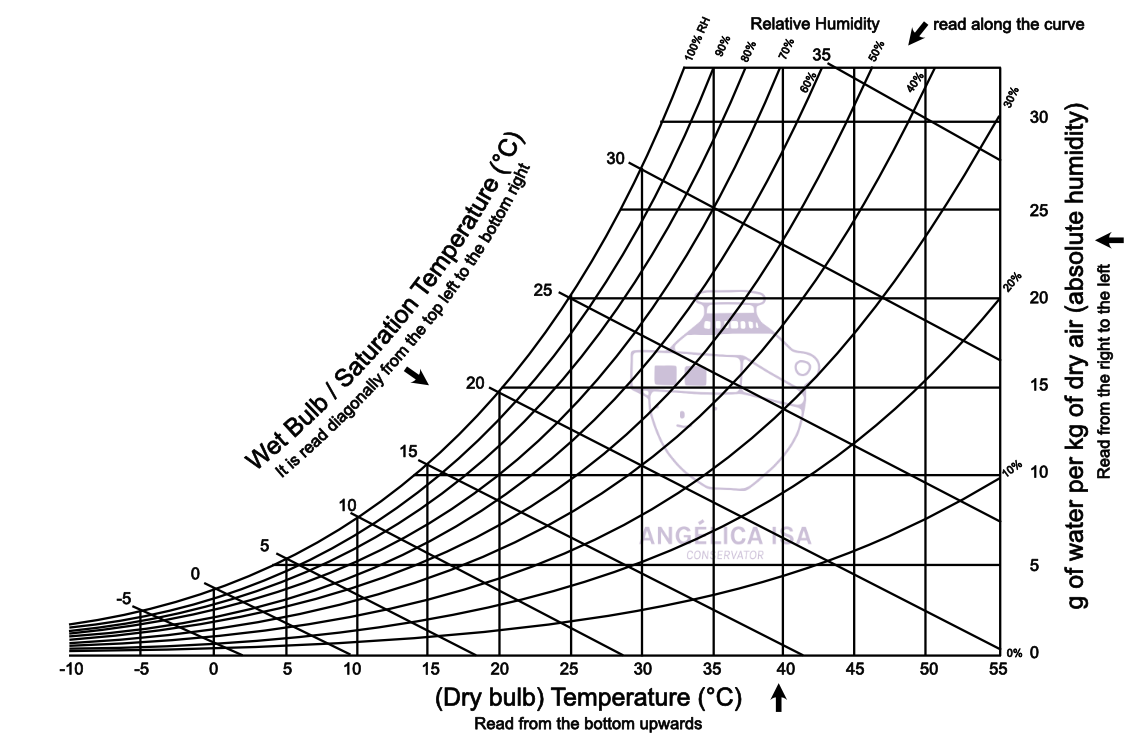
\includegraphics[width=0.95 \textwidth]{images/08_psychrometric_angelica-isa.png}\\
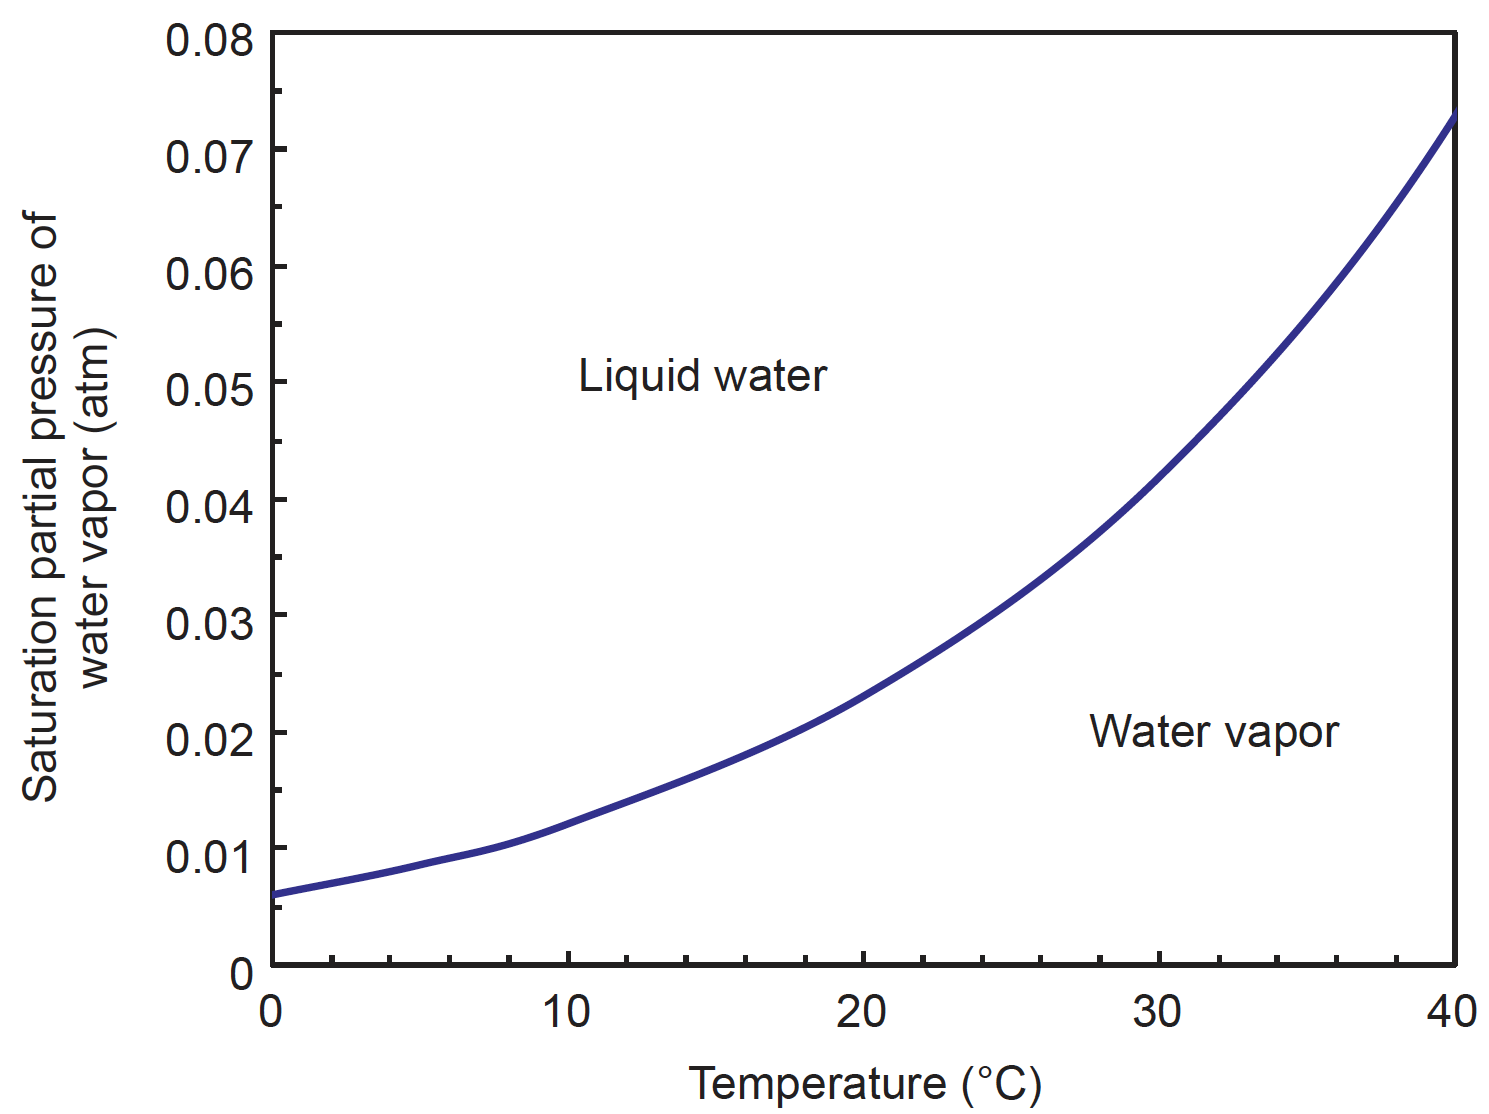
\includegraphics[width=0.95 \textwidth]{images/08_pressure-vs-temperature-clausius-clapeyron_mathez-fig-1-2_no-caption.png}
\caption{ \label{fig:08_psychrometric-and-phase-diagrams}
{\bf Top}: Psychrometric chart for water at standard pressure conditions $\unit{1}{atm} = \unit{101}{\kilo\pascal}$ (from angelicaisa.com). {\bf Bottom}: Phase transition coexistence curve for water near the triple point (from Mathez \& Smerdon).
}
\end{figure}



\newpage
%%%%%%%%%%%%%%%%%%%%%%%%%%%%%%%%%%%%%%%%%%%%%
%%%%%%%%%%%%%%%%%%%%%%%%%%%%%%%%%%%%%%%%%%%%%


%%%%%%%%%%%%%%%%%%%%%%%%%%%%%%%%%%%%%%%%%%%%%
\section{Experiments and Analysis}

{\bf \underline{Safety Notes}:} 
	%
	\begin{itemize}
	\item For the ``cloud chamber'' experiment, your instructor will provide you with a chunk of solid carbon dioxide (``dry ice'').  This is about $-80\degree$C and it will burn you if you touch it. So,  please {\bf use the thermal gloves to handle the dry ice} if you need to (but you probably won't need to handle it).
	\item Also for the cloud chambers, you will be provided with a small radioactive rock (containing uranium and other things).  As we will see, this emits ``alpha particles'' (helium nuclei). These particles are not able to penetrate your skin and are therefore safe.  However, you would not want to consume these rocks as the alpha particles could damage you internally.  So do not eat the radioactive rock, and also {\bf do not touch the radioactive rock without nitrile gloves}.  If you do happen to touch the rock, then wash your hands carefully.
	\item We can use smoke from a match to stimulate ``nucleation'' of clouds from the water vapor.  Be sure to keep your match strkes far separated from the isopropanol (alcohol), which is very flammable.
	\end{itemize}

\subsection{Observing the dew point and frost point}

We will not be performing our experiments outside, so we need to calculate the partial pressure of water for the conditions in this room.  Measure the temperature of the room with the IR thermometer gun (look at a bunch of objects that should be in thermal equilibrium with the air), and the relative humidity using the hygrometer.  Also give uncertainties for these measurments (and your rationale for these values).

\answerspace[3.5cm]

\noindent Use the process from the introduction, and your equation for $f$, to convert your relative humidity value to an absolute humidity (AH) and finally to a partial pressure, $e$, in atmospheres.  Then use the coexistence curve in the phase diagram (Fig \ref{fig:08_psychrometric-and-phase-diagrams}) to determine the vaporization temperature (the dew point) in this room.  Record the value and any intermediate calculations here.

\answerspace

\noindent Put some ``cold'' tap water in a 250~mL beaker; measure and record its temperature.  Then slowly add ice to the water to reduce its temperature.  Observe what happens to the outer walls of the beaker, noting the temperature(s) at which any changes occur.  Record your observations here and give an explanation for what is occuring.

\answerspace

\noindent If you examine the full phase diagram from last week  (Figure \ref{fig:07_phase-diagram-water}),  you see that the coexistence curve between liquid water and solid water is basically vertical, meaning it has the same transition temperature regardless of the pressure value.  What does this means for ``freezing of liquid water exposed to air'' (as compared to our discussion above of evaporation while boiling, pure water vs.\ surface water)?

\answerspace[3cm]  

\noindent Try to observe this {\bf frost point} by cooling your water further (this can be accomplished by adding salt to the water, since ``freezing point depression'' lowers the transition temperature within your beaker, allowing the water-salt-ice mixture to go below 0$\degree$C). Record any observations and temperature measurements.

\answerspace


\subsection{Drying your hands}

You are familiar with washing your hands and letting them dry off.  Let's try to quantify that experience, slightly.  Measure the temperature of ``cold'' water from the tap. Then run your hands under the water for a few seconds.  Turn off the water and shake off your hands five times to remove large water droplets.  Now wave your hands back and forth in the air in a regular motion while your partner times you with a stopwatch. Stop the timer when your palms are dry, as determined by your partner.  Repeat the whole experiment with ``hot'' water from the tap.   Record your temperatures, times, and observations here.


\answerspace

\noindent You likely found a measureable difference between the two cases. Why do you think that is the case? How can it be explained physically?

\answerspace


\subsection{An alcohol upside-down cloud}

Particle physicists use ``cloud chambers'' to observe the paths of particles in nuclear reactions (e.g., the break-up of atoms into smaller atoms by fission) and particle collision experiments.  We will build such a chamber using isopropyl alcohol (isopropanol).  The reason that alcohol is used is because it actually {\em does not} make clouds easily: it does not {\bf nucleate} as easily as other substances, meaning that vapor will remain vapor below the liquid-vapor transition temperature if there are no good ``seeds'' on which to form water droplets.  A {\bf cloud} is actually not composed of vapor, but is instead small liquid or ice droplets that have formed when vapor cools and condenses.  So, in the cloud chambers we will build (and that particle physicists use) the air is {\em super saturated} with alcohol and makes a ``cloud'' (the trail of tiny liquid particles) only when driven to nucleation by the ionization of air/alcohol from the passing nuclear decay particles (alpha particles, i.e., Helium nuclei).\\[-6pt]

\noindent {\bf Procedure:} 
	%
	\begin{itemize}
	\item Construct your cloud chamber by doing the following: (1) Fold a piece of felt in half and cut it so that the folded piece matches the base of the cubical box. (2) Attach the felt to inside bottom of the box using magnets. (3) Cover the bottom of the baking pan with black acrylic (4) Soak the felt with alcohol; it should be wet, but there should not be excess liquid in your box when you turn it upside down (if there is, pour that out). (5) Place a radioactive rock at the center of your upside-down baking sheet (your instructor will bring it over using gloves). (6) Turn your baking sheet upside down (acrylic side up); place a small radioactive rock on the center of the sheet (using gloves); and then place the cloud box upside-down onto the baking sheet. (7) Seal the bottom edge of the box to the baking sheet using caulk and the caulk spreader, all the way around the four edges.  (8) Place a chunk of dry ice (your instructor will bring it over using thermal gloves) on the corkboard mat and place the baking sheet  with box on top of the dry ice, so that the black ``floor'' of your box is cold.
	\item The clouds are best observed in a mostly dark space, using a flashlight. Look for ``streams'' of cloud emerging from the radioactive rock.  Try to take a video of it with your phone or the go-pro camera.  The particles should be leaving the rock with high velocity generating a straight-line cloud, which then sinks and floats away.  Can you catch an image straight-line cloud?
	\item As noted above, the alcohol does not nucleate well, so although its temperature is below the vaporization temperature (in the region near the dry ice base) it remains vapor (until the alpha particle causes an ionization trail).  You can force the alcohol to nucleate by lighting a match, letting it go out, collecting the smoke with the syringe, and then pumping smoke into the box through its tube.  Just a small amount of smoke should lead to a much larger volume of ``cloud.''  The smoke provides aerosol particles as nucleation sites.  Once you add the smoke, you will not likely see the radioactive emissions anymore.
	\end{itemize}
	%
Draw your setup and describe your observations.  

\answerspace[7cm]
	
\noindent Describe the entire process by which the clouds are formed here, starting with the liquid alcohol in the felt.  Make clear what is seen and what is invisible.

\answerspace[7cm]

\subsection{Cloud convection}

Now we will build clouds made of water vapor.  The reason the alcohol clouds were ``upside down'' (the alcohol was placed on the ceiling, the clouds formed down at the cold bottom layer) was because alcohol vapor is {\em more dense} than air and therefore sinks.  Water vapor, however, is {\em less dense} than air, so once formed it will rise in air. In our enviroment outside, water evaporates off of  lakes and oceans and then rises upwards.  When the temperature drops sufficiently, the water vapor (invisible) becomes liquid or ice droplets forming a cloud that can be seen.  In this experiment, we will partially fill a jar with warm water and then create a cold ``roof'' that is is a bit below 0$\degree$C. This actually perfectly matches the warm climate we experience at Earth's surface and the colder temperatures you would measure going vertically upward in the atmosphere.\\[-6pt]

\noindent {\bf Procedure:}
	%
	\begin{itemize}
	\item We will construct water vapor clouds in glass jars (either short or tall; you will have a chance to experiment).  The basic setup will be: warm tap water in the bottom of the jar; a bowl of salted-ice slurry\footnote{A {\em slurry} is a mixture of denser solids suspended in liquid, usually water; here we dissolve and suspend salt.} sitting on the lid; a flashlight to observe any convection; small amounts of added smoke to force nucleation and visible clouds.
	\item Create your salt-ice slurry by filling a 500~mL beaker with ice and adding a lot of salt.  Start stirring it vigorously and the ice will begin to melt forming a water-ice-salt mixture at the bottom.  You don't want too much water because you are relying on the the very cold (-20 to -10$\degree$C) ice to bring the mixture below the freezing point of water. So try to avoid adding water.  Use your thermometer to monitor the temperature of your slurry.  You can pour out water and add ice to keep it getting colder.  You should be able to easily produce a slurry of -10$\degree$C or lower.
	\item Get warm or hot water ($\sim40\degree$C) from the tap and fill the jar with about an inch of water.  
	\item Put slurry in the small glass bowl and fit it into the open lid of the jar.
	\item Turn off the lights and observe with a flashlight.  You should start to see ``convection'' rolls as the water vapor evaporates off the warm water surface, rises quickly and then condenses and cools near the top, falling as colder air or vapor.  
	\item Like the alcohol cloud chamber, you can force nucleation by adding some aerosol particles.  Light a match and blow it out, lift the bowl and wave a small amount of smoke into the jar.  Again you should see more cloud formed than just the smoke that you added, since the smoke acts as a nucleation site for cloud (as well as being visible itself as a tracer). Try to add a small amount of smoke at first.  You can always blow out your jar and re-start.
	\end{itemize}
	%
Draw your setup and describe your observations.  

\answerspace[7cm]
	
\noindent Describe the entire process by which the clouds are formed here, starting with the liquid water in the base of the jar.  Make clear what is seen and what is invisible.

\answerspace[7cm]


\subsection{Less convective clouds}

Since these water-vapor cloud jars are easy to make and adjust, we can try to vary the parameters to alter the conditions of the cloud formation and equilibrium.  The conditions for the previous setup included a large temperature gradient between the liquid ($\sim40\degree$C) and the cold ceiling ($\sim-15\degree$C).  This large difference should have led to a rapid rolling convection of the atmosphere in the jar.  Here we would like to adjust the setup to try to obtain clouds with less convection, i.e., a more stable layer of clouds.  \\[-6pt]

\noindent Discuss the relevant temperatures and heights involved in the formation of clouds in our atmosphere.  You can look up information if you need to, and you might also recall (or go outside an measure) the IR thermometer gun measurements of the sky and cloud base.  Specifically: What temperature is the water from which vapor is evaporating (of course this depends where on Earth you consider)? What is the height at which clouds are formed?  What temperature is the air at the height where clouds are formed?

\answerspace[7cm]

\noindent Consider how you might scale the atmospheric scenario down to your jar.  Parameters that you could vary are: (i) height of the jar (we should have two heights available), (ii) temperature of the water, and (iii) temperature of the ceiling.  Detail here one or more experimental procedure to create a new cloud-in-jar to realize this scaled-down atmosphere.  

\answerspace[7cm]

\noindent Perform one or more of your experiments and detail your observations.

	

\answerspace[7cm]



 

%%%%%%%%%%%%%%%%%%%%%%%%%%%%%%%%%%%%%%%%%%%%%
%                        Week 09  ---  Milankovitch (no lab in F2025)
%%%%%%%%%%%%%%%%%%%%%%%%%%%%%%%%%%%%%%%%%%%%%


%%%%%%%%%%%%%%%%%%%%%%%%%%%%%%%%%%%%%%%%%%%%%
%                        Week 10  ---   IR aborption by Greenhouse Gases
%%%%%%%%%%%%%%%%%%%%%%%%%%%%%%%%%%%%%%%%%%%%%



\ChapterWithSubtitle{IR Absorption by GH Gases (F25: 2 Weeks)}{I am back to save the universe}
%\chapter{Heating by Radiation}

%%%%%%%%%%%%%%%%%%%%%%%%%%%%%%%%%%%%%%%%%%%%%
\section*{Equipment List}

\begin{multicols}{2}   % change 2 -> 3 for three columns
\begin{equipment}
\item Ruler
\item Digital Thermometer
\item Sharpie
\item 250 mL beaker 
\item 500 mL beaker 
\item Hot Plate
\item Lab jack
\item IR thermal imaging camera
\item IR thermometer
\item plastic basket with windows
\item Voltage amplifier box and wires
\item Cardboard box ``tunnel'' for restricting thermopile's field of view
\item Digital multimeter (DMM)
\item Various narrow-band thermopiles (\unit{3.375}{\micro\meter}, \unit{3.91}{\micro\meter}, \unit{4.3}{\micro\meter}, \unit{4.43}{\micro\meter}) and a broad-spectrum thermopile (\unit{8}{\micro\meter} -- \unit{14}{\micro\meter})
\item ziploc-style  bags (for classroom)
\end{equipment}
\end{multicols}


%%%%%%%%%%%%%%%%%%%%%%%%%%%%%%%%%%%%%%%%%%%%%
\section{Introduction and Definitions}

\subsection{Climate Sensitivity}

This week in class we are attempting to identify the precise connection between additional greenhouse gases in the atmosphere and the resulting temperature increase.  This connection is called the {\bf climate sensitivity}\footnote{{\em Climate sensitivity} is often used as a technical term by climate scientists to refer to ``the temperature increase due to a doubling of atmospheric $\text{CO}_2$''; but it is also used in this more general sense.}.  In lecture and discussion, we will attempt to see this connection through the deepening and broadening of $\text{CO}_2$ absorption lines in the blackbody spectrum of the Earth surface's infrared radiation. Here, in lab, we will simply try to quantitatively observe the absorption of infrared light by $\text{CO}_2$ (and possilbly air and water vapor).

\subsection{Absorption lines and IR thermometer/camera measurements}

Previously in Discussion we learned how to draw blackbody spectra on log-log paper and then, when studying the IR absorption by greenhouse gases, we sketched absorption lines on these spectra.  Recall the relevant equations for this process:
	%
	\begin{equation*}
	\lambda_\text{peak} = \frac{\unit{2900}{\micro\meter \cdot \kelvin}}{T}  \quad ; \quad
	F = \left( 5.7 \times 10^{-8} \, \frac{\text{J}/\text{s}}{\text{m}^2 \cdot \text{K}^4}\right) T^4 \quad ; \quad
	F_\lambda = \frac{F}{1.5 \times \lambda_\text{peak}}
	\end{equation*}
	%
To create the blackbody curve, we drew the peak (``hat'') with three points at wavelengths of $[ \frac{\lambda_p}{2}, \lambda_p, 3 \lambda_p]$, and at spectral flux values of $[\frac{F_\lambda}{10}, F_\lambda, \frac{F_\lambda}{10} ]$; the curve dropped off with a slope of 4 to high wavelengths, and more quickly at low wavelengths.\\[6pt]

\noindent On a single piece of log-log graph paper, draw blackbody curves for the following temperatures: room temperature ($20\degree\text{C} = \unit{293}{\kelvin}$); hot water ($50\degree\text{C} = \unit{323}{\kelvin}$); boiling water ($100\degree\text{C} = \unit{373}{\kelvin}$); and a heat lamp at $450\degree\text{C} = \unit{673}{\kelvin}$. Make your calculations here:


\answerspace[7cm]

\noindent We will attempt to see the absorption of infrared light by carbon dioxide using IR thermometer guns and imaging cameras, but this is not a completely straightforward process because of how these devices work.  First, they estimate temperature by collecting all light over a range of wavelengths, 8--\unit{14}{\micro\meter}.  They measure the total flux emitted by an object in that wavelength range and then compare it to what would be expected from blackbody curves at different temperatures (the ``area under the curve'' between these wavelengths).  On your blackbody graph, draw two vertical lines to indicate this range of wavelengths.  Looking at your curves, which of the objects would have the most flux in this range.  Can you estimate how much more\footnote{An approximation to the observed total flux is the area of a rectangle that has height $F_\lambda$ (at the center of the 8--\unit{14}{\micro\meter} interval) and width: $\unit{14}{\micro\meter} - \unit{8}{\micro\meter} = \unit{6}{\micro\meter}$.} it is than the second most?

\answerspace

\noindent A second issue with these devices is that their wavelength range has been specifically chosen to {\em avoid} the $\text{CO}_2$ absorption lines, which (remember from our {\em Infrared Absorption} discussion) are at \unit{4.3}{ \micro\meter} and \unit{15}{\micro\meter}.  Draw vertical lines on your blackbody curve to indicate these wavelengths.  Is it possible that a carbon dioxide absorption line will affect anything in the 8--\unit{14}{\micro\meter} sensitivity range of the devices?  Why or why not?

\answerspace

\noindent We do expect to see some small effect because of the line width of carbon dioxide, particularly at \unit{15}{\micro\meter}.  As that line takes a bite out of the spectrum, it should cover a small part of the sensitivity range of the devices.  Sketch absorption ``valleys'' on each of your spectra at both the \unit{4.3}{\micro\meter} and  \unit{15}{\micro\meter} locations.  Looking at your graphs, do you expect that any of the three non-room-temperature sources would be more affected\footnote{I don't think there is a clear-cut answer to this, particularly from our approximate blackbody curves, but it is an interesting question to think about.} than others?



\newpage
%%%%%%%%%%%%%%%%%%%%%%%%%%%%%%%%%%%%%%%%%%%%%
%%%%%%%%%%%%%%%%%%%%%%%%%%%%%%%%%%%%%%%%%%%%%


%%%%%%%%%%%%%%%%%%%%%%%%%%%%%%%%%%%%%%%%%%%%%
\section{Experiments and Analysis}

{\bf \underline{Safety Notes}:} 
	%
	\begin{itemize}
	\item We have tanks of $\text{CO}_2$ and $\text{N}_2$ gas in the classroom.  Do not disturb their buckle attachments to the table as the greatest danger would be for them to fall, break a valve and then ``rocket'' across the room.  Be gentle when screwing the valves to release the gases.
	\item We will use a hot plate as a thermal radiation source. It is hanging vertically, so be careful not to touch or brush up against it.
	\end{itemize}
	
\noindent As always: \underline{read the full procedures} prior to beginning any experimentation.

\subsection{IR transparency of plastic bags}

Make some measurements and observations to test  transparency of the plastic bags we will later fill with gas.  There are multiple types of bags that can be used (multiple ``Ziploc''-style, and food-storage ``produce'' bags). You can use IR thermometer gun and the IR imaging camera.  Observe what is visible in the camera image and how the measurements of temperature recorded by both devices changes through one or multiple plastic bag layers.  You can use humans as sources of IR or fill a beaker with ``hot'' tap water.\\[-6pt]

\noindent Record your observations, measurements, and conclusions here.

\answerspace[7cm]


\subsection{IR absorption in air}

Complete the steps below with your table of four using the Mileseey infrared camera. We are interested in the device's measured temperature of the vat of water at different distances, but because it is cooling in the room over time, we need to observe that cooling for a few minutes at each distance and then extrapolate backwards to obtain an estimate of the initial temperature for each distance. \\


%%%%%%%%%%%%%%%%%%%%%
\newpage

\noindent {\bf Procedure:} 
	%
	\begin{itemize}
	\item Starting at the vat of hot water (tap water at $\sim 50\degree$C), use a meter stick (located along the walls on top of the power strip) to mark out  distances of \unit{1}{\meter}, \unit{2}{\meter}, \unit{3}{\meter}, \unit{4}{\meter}, and \unit{5}{\meter} with masking tape on the floor.
	\item Start your stopwatch.
	\item Use the IR camera to make measurements of the temperature of the vat of water from zero to five meters, recording the time, distance, and temperature. You should be able to use the (red) ``max'' temperature value shown on the image (or the white central cross-hairs temperature shown at top left).  These measurements will probably be 20--30 seconds apart. Enter these values in a three-column table in Google Sheets, recording the time in two columns, minutes and seconds, so that you can later convert to ``t (s)''.
	\item Repeat the zero to five meter measurements 5--7 times.
	\end{itemize}
	%

\noindent {\bf Analysis:} Copy the Google Sheets table for each student. Using the two time columns, create a ``time in seconds'' column (with an excel command like ``\verb|=A2*60+B2|'').  On a single sheet of graph paper, plot six data sets for the Temperature vs.\ time values at each distance (make each axis range as narrow as possible while still showing the data \ldots it is not necessary to show the ``origin'').  [Alternatively you could copy your data into separate sheets for each distance and insert Charts for each.]  Using a ruler, draw a line of best fit and obtain the ``y intercept,'' i.e., the temperature at time zero, for each of the datasets.  Then make a new plot, on another sheet of graph paper, showing initial temperature vs.\ distance.\\[-6pt]

\noindent Briefly state what you observe in each of the two graphs.  How do your results demonstrate absorption of IR light, if at all?  If there is IR absorption, what do you think is the primary contributor?

\answerspace

\vfill

--- End of Day 1 ---

%%%%%%%%%%%%%%%%%%%%%
\newpage


\subsection{IR absorption by $\text{CO}_2$ (effect on reported temperature)}

We will use a hot plate for our infrared radiation source and observe the reported temperature by an IR thermometer gun through bags of gas. You can set the hot plate to the max temperature value or, following your analysis in the introduction of blackbody curves and absorption lines, choose a different temperature of the source.  You will observe this source through three bags of gas: first all three nitrogen; then replacing each nitrogen, one-by-one, with carbon dioxide.  Then you will repeat this process using bags of air. You will measure the temperature of the source through the bags in each case and seek some effect of carbon dioxide absorption.  \\[-6pt]

\noindent {\bf Procedure:}
	%
	\begin{itemize}
	\item Set up your hot plate vertically,  turn it on, and set its temperature.
	\item Using the tanks of $\text{CO}_2$ and $\text{N}_2$ gas, fill three clear quart-size, ziploc-style bags of each gas (avoid bags if the lettering/logo blocks the line-of-sight). Label each at the bottom of the bag using a Sharpie, indicating its contents.  When using the tanks: the main tank valve should be {\em unscrewed} (CCW) a little bit from the closed position.  Then the secondary valve (thin bar) is {\em screwed in} (CW) to make the gas come out. Your instructor will help you with this. Be gentle with the screwing and unscrewing, and try not to let too much gas escape when filling. Fill the bags up as full as you can. When finished, close the tank valves again.
	\item Fill three more bags with air from the room, using the small orange pumps. [Alternatively, you could use your breath to fill these bags, which will contain a higher concentration of $\text{CO}_2$ than air ($\sim 3\%$ rather than $0.0425\%=\unit{425}{ppm}$), and possibly some water vapor.]
	\item Place your windowed basket on the lab jack and point it toward the hot plate source.  Place blue masking tape on the table to record the distance of your basket from the hot plate; measure that distance and record it.  To avoid burning the bags/basket, this should not be too close, probably around \unit{40}{\centi\meter}.  Once your hot plate has reached a constant temperature as measured by your thermometer gun, record both the hot plate temperature setting and the actual temperature.
	\item Create a table, on paper or Google Sheets, to record temperature measurements.  You should have four columns: [$N_{\text{CO}_2}$, $N_{\text{N}_2}$, $N_\text{air}$, $T$], to express the combination of bags.
	\item First record the temperature of the hot plate through the window of your empty basket. Be sure hold the trigger down, and scan the hot plate slowly to find the hottest point.  You will always record this maximum temperature.
	\item Then, start with three bags of nitrogen.  Make sure the bags are puffed up fully, e.g., by holding your hand flat across their tops if the bags are not completely full on their own. Also make sure the line of sight through the basket windows is pointed at the hot plate and there are no obstructions (e.g., folds/seams in the ziploc bags or  Record the temperature through the bags in your table.
	\item Replace one nitrogen bag with a carbon dioxide bag.  Again record the temperature.  Then replace another $\text{N}_2$ bag with $\text{CO}_2$ and repeat. Record your measurements in a table with columns noting the number of $\text{N}_2$ and $\text{CO}_2$ bags ($N_\text{air}$ will be zero for all of these measurements).
	\item Return to three nitrogen bags and then replace them sequentially with the air bags.
	\item Turn off your hot plate.
	\end{itemize}
	

\noindent {\bf Analysis:}   Make two graphs:  temperature vs carbon dioxide bag number, and temperature vs.\ air bag number. In the space below, describe what you have seen and decide if you have observed any absorption by carbon dioxide (or in the case of the air bag, absorption by either carbon dioxide or water vapor).

\answerspace[8cm]

\noindent Why did we use nitrogen as the comparison gas?

\answerspace


%\subsection{IR absorption by wet $\text{CO}_2$ (OPTIONAL)}
%Repeat the prior experiment, but filling the bags with carbon dioxide generated with baking soda and vinegar.

\subsection{IR absorption by $\text{CO}_2$  (an absorption spectrum)}

With your table of four, you will now attempt to see the wavelength dependence of infrared absorption by $\text{CO}_2$. We will again use the hot plate as the IR source, this time at maximum temperature.  We have a collection of four narrow-band infrared {\em thermopiles} (the same detector that is used within the thermometer guns, but restricted to a very narrow wavelength band around their central value, rather than $8$--\unit{14}{\micro\meter}), as well as a broad-band thermopile for comparison. These thermopiles output a miniscule voltage (in the hundreds of microvolts range) which we can amplify into hundreds of millivolts and observe with the digital multimeter (DMM).  We will again compare observations through bags of nitrogen, carbon dioxide, and air; but this time using only a single bag held in front of the thermopile. \\[-6pt]

%%%%%%%%%%%%%%%%%%%%%
\newpage

\noindent{\bf Equipment Notes}:
	%
	\begin{itemize}
	\item The DMM should be set to voltage (the ``$\text{V}\sim$'' selection) on the dial, and then switched to ``DC'' voltage (from the ``AC'' default) by pressing ``Select'' button.  If the DMM powers off while using, press the Select button once to turn back on, and again to switch to DC voltage.
	\item The wire leads from the DMM will be directly connected to the various thermopile squares (red to red, black to black). Readings on the DMM from these devices will be small and often negative. This is ok, since only differences in voltage have physical meaning. High voltage values (e.g., less negative values) will correspond to higher infrared intensity. Be sure to include the sign of your voltage reading when recording data.  
	\item The connections of the DMM and the power source should be set up for you already, but ask your instructor if you have trouble getting readings, or think it might have been disconnected.
	\end{itemize}

\noindent{\bf Procedure}:
	%
	\begin{itemize}
	\item Set up using the hot plate that is facing away from the nearest wall so that you will point your thermopiles away from the center of the room (they are very sensitive to stray infrared light sources, like people). Turn on the hot plate and set to maximum temperature.
	\item Select nice plump bags of nitrogen, $\text{CO}_2$, and air, one bag for each gas.
	\item Create a Google sheet, with columns for: 
		%
		\begin{quote}
		[$\lambda$, Vhp (no bag), Vhp (N2), Vhp (CO2), Vhp (air), Vw (no bag)]%, Vw (N2)]
		\end{quote}
	where ``V'' stands for voltage, ``hp'' stands for hot plate (measurements pointed at the hot plate), and ``w'' stands for wall (baseline measurements pointed at the wall, at approximately room temperature). There will be five rows --- one for each narrow-band thermopile, and one broadband (8--\unit{14}{\micro\meter}) --- with wavelength $\lambda$ values \{3.375, 3.91, 4.3, \unit{4.43}{\micro\meter}\}.
	\item Set the cardboard box tunnel on the top of the lab jack and raise it such that the box is pointed at the center of the hot plate.  Attach binder clips to the sides of the back of the lab jack platform and push the ends of the red and black wire leads through the binder clips (so the wires are ready to be plugged into a thermopile).  
	\item This time, the lab jack can be about \unit{20}{\centi\meter} away from the hotplate when making measurements (since we will not leave bags near the hot plate). Set its distance, measure it, and place tape on the table so that it can be easily positioned.  Before measurements it can be moved away to avoid getting too hot.
	\item Once the hot plate has reached a steady temperature, record its stated value and the actual value measured with the infrared thermometer gun.
	\item Select one of the five thermopiles from the thermopile library provided to the class as a whole. Attach the red and black wires to it and push it into the ``back window'' of the cardboard box (the one that goes to the bottom).
	\item Recording voltage measurements: (i) prop the DMM on its stand so that it can easily be read; (ii) have one person stand very still to the side of the table, ready to hold bags between the box window and the hot plate; (iii) try to keep everyone else out of the field of view of the sensor (or the ``reflection'' off the hot plate \ldots check out your own reflection in the aluminum baking sheet, using the thermal imaging camera!).
	\item Wait for the voltage reading to stabliize and record the ``Vhp (no bag)'' measurement.  Then hold the nitrogen bag in front of the ``front'' window of the cardboard box, wait for the voltage reading to stabilize, and record it.  Repeat for all other columns.  For the ``wall'' columns, move the lab jack away from the hot plate and point your sensor at the room-temperature wall.
	\item Switch to a different thermopile sensor and collect its data in the next row of your Sheet.
	\end{itemize}


\noindent {\bf Analysis:}   Because each sensor has a slightly different wavelength width and base voltage value, we will make a ``spectrum'' (for the carbon dioxide and air bags) by normalizing their values to the nitrogen values.  Make three new columns in your Google Sheet for the ``normalized voltages'', titled [VnN2, VnA, VnCO2]. The equation to get each of these values will be:
	%
	\begin{equation*}
	V_{\text{norm}, \text{gas}} = \frac{ V_{\text{hp}, \text{gas}} - V_{\text{wall (no bag)}} }{ V_{\text{hp}, \text{N}_2} - V_{\text{wall (no bag)}} }
	\quad \quad \left( \text{with ``gas'' } = \text{ N}_2, \text{CO}_2, \text{air}\right)
	\end{equation*}
	%
Explain what this equation means, in your own words.  What will be the value for each of the $\text{N}_2$ normalized voltages?

\answerspace

\noindent You can implement this equation using an Excel-style formula in your Google Sheet.  If the data for one thermopile is in row 2, with $\lambda$ in column A (and the voltage values listed above in the next columns), then a formula like this should work for the normalized $\text{CO}_2$ value:
	%
	\begin{quote}
	\verb| = (D2 - F2) / (C2 - F2) |
	\end{quote}
	%
Explain why this (or something close to it for your Sheet) matches the above equation for normalized voltage and the columns listed within the Procedure.

\answerspace


\noindent Type in the Excel formula for the first row in each of the normalized voltage columns; then drag the bottom right corner of the cell down to fill the values for all other thermopile rows. What do you see for the normalized voltages in the ``broadband'' (8--\unit{14}{\micro\meter}) thermopile?  Since this is the sensor in the IR thermometer guns, does this data support your findings from the prior experiments?  Why or why not?

\answerspace

\noindent Plot the normalized voltages vs.\ wavelength for $\text{N}_2$, $\text{CO}_2$, and air together on one (scatter) Chart (using only the narrow-band thermopiles, not the broadband). To make a Chart that displays multiple data sets, copy your single table into multiple copies in the manner shown in the figure below (Source: \href{https://www.reddit.com/r/googlesheets/comments/17sm8q5/comment/k8qyb0j/}{Reddit user 7FOOT7}). Notice that you should have three different rows with the same wavelength, one for each column of normalized voltages.  Highlight that full dataset, including its column labels (so it would be \verb|A1| to \verb|D10| in the example below), and do {\em Insert}/{\em Chart}.
%
\begin{center}
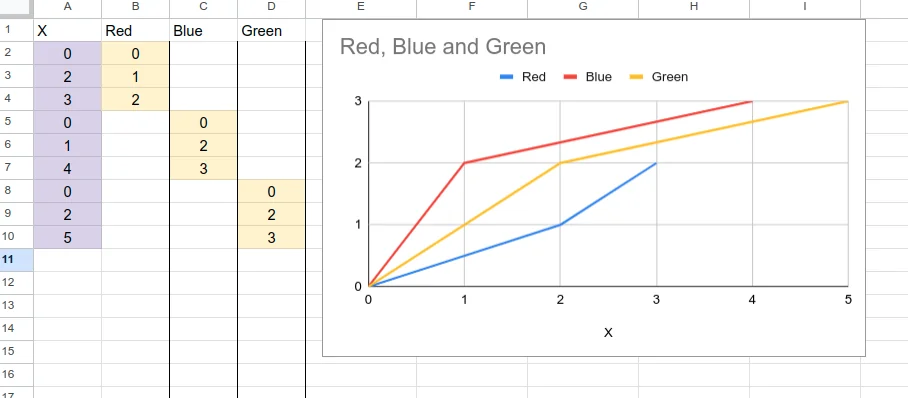
\includegraphics[width=\textwidth]{images/09_multiple-lines-on-chart-google-sheets.png}
\end{center}
%
What do you see in your spectrum?  Is there evidence of absorption by $\text{CO}_2$? How does the ``air'' spectrum compare to the $\text{CO}_2$ spectrum?  Try to give an explanation for the results in terms of what we have learned about greenhouse gases in other parts of the course.

\answerspace[5.5cm]

\noindent If you examine your data, comparing the ``Vhp (N2)''  and ``Vhp (CO2)'' raw values to the ``Vhp (no bag)'' values, you should see that there is one wavelength for which: (i) nitrogen and carbon dioxide have similar values, but (ii) both nitrogen and carbon dioxide are lower than at other wavelengths.  [If you would like, you can create another graph to see this clearly, by creating a normalized spectrum (now for $\text{CO}_2$, air, and $\text{N}_2$) to the ``Vhp (no bag)'' rather than to nitrogen.]  Do you see this? What is the explanation?





%{\em [F2025] We have an array of five narrow-band infrared sensors (thermopiles) from which one can measure input radiation as a voltage.  By comparing the radiation incident on the sensors through bags of nitrogen to that through bags of carbon dioxide, we can obtain an approximate spectrum showing the absorption line around \unit{4.3}{\micro\meter}.  Unfortunately we do not have the technical details of this experiment ready yet.  We will potentially revisit in a future week.}
	

\answerspace[7cm]



 



%%%%%%%%%%%%%%%%%%%%%%%%%%%%%%%%%%%%%%%%%%%%%
%                        Week 11  ---  Forcings and Timescales of Climate Change
%%%%%%%%%%%%%%%%%%%%%%%%%%%%%%%%%%%%%%%%%%%%%

%%%%%%%%%%%%%%%%%%%%%%%%%%%%%%%%%%%%%%%%%%%%%
%                        Week 12  ---  Modeling Climate Change
%%%%%%%%%%%%%%%%%%%%%%%%%%%%%%%%%%%%%%%%%%%%%


\ChapterWithSubtitle{Modeling Climate Change}{now we can swim any day in november}
%\chapter{Heating by Radiation}

%%%%%%%%%%%%%%%%%%%%%%%%%%%%%%%%%%%%%%%%%%%%%
\section*{Equipment List}

\begin{multicols}{2}   % change 2 -> 3 for three columns
\begin{equipment}
\item Computer (lab-provided or your own)
\end{equipment}
\end{multicols}


%%%%%%%%%%%%%%%%%%%%%%%%%%%%%%%%%%%%%%%%%%%%%
\section{Introduction}

Today we will explore an online climate simulation tool, called {\bf En-ROADS}\footnote{\url{https://en-roads.climateinteractive.org/scenario.html}}, created by MIT Sloane School of Management and the ``environmental think tank''  \href{https://www.influencewatch.org/non-profit/climate-interactive/}{\em Climate Interactive}. You should have watched their 10~min ``Overview and Introduction'' video\footnote{Located in 2025 at \url{https://www.youtube.com/watch?v=4O-5fsVZaII}} already, but you could refresh yourself now with the 2~min ``Overview'' video at {\em Help/Video Tools/EN-ROADS Overview}\footnote{We will explore this tool and try to become familiar with it, but if you would like to train yourself more deeply you could take their online course \url{https://learn.climateinteractive.org/course/mastering-en-roads}.}.  Your reading this week from Dessler (Chapter 8: {\em Predictions of Future Climate Change}) will also help you to understand the definitions and methods of quantities used in this modeling tool.

To get started, take 10--15 min to play with the tool, exploring the options for adjusting the parameters (both using the adjustable bars, and opening the setting to manully control the numbers), visualizing different output graphs, and determining outcomes that differ from the ``baseline'' presented.  Talk with the lab partners at your table about what you are finding and share methods on how to access all of the tools/options.  While/after doing so, write a brief paragraph that answers most of the following questions.
	%
	\begin{itemize}
	\item What is the basic idea of this tool?  What are the inputs and what are the outputs?
	\item Where are the connections to our prior study of climate change, e.g., ``climate sensitivity'', the connection between increasing $\text{CO}_2$ in the atmosphere and temperature rise?
	\item What else is incorporated in the tool, other than these climate physics principles?  (I would say it accounts for the science, but also societal and economic factors. How?)
	\item Explain the plot shown in the 10~min En-ROADS introduction video (at 4:54, reproduced below), in which En-ROADS is compared to NGFS.  What does the graph show? What is NGFS and why are they comparing to it? What are the three different scenarios plotted? (You might need to look some things up online!)
	\end{itemize}

\vfill

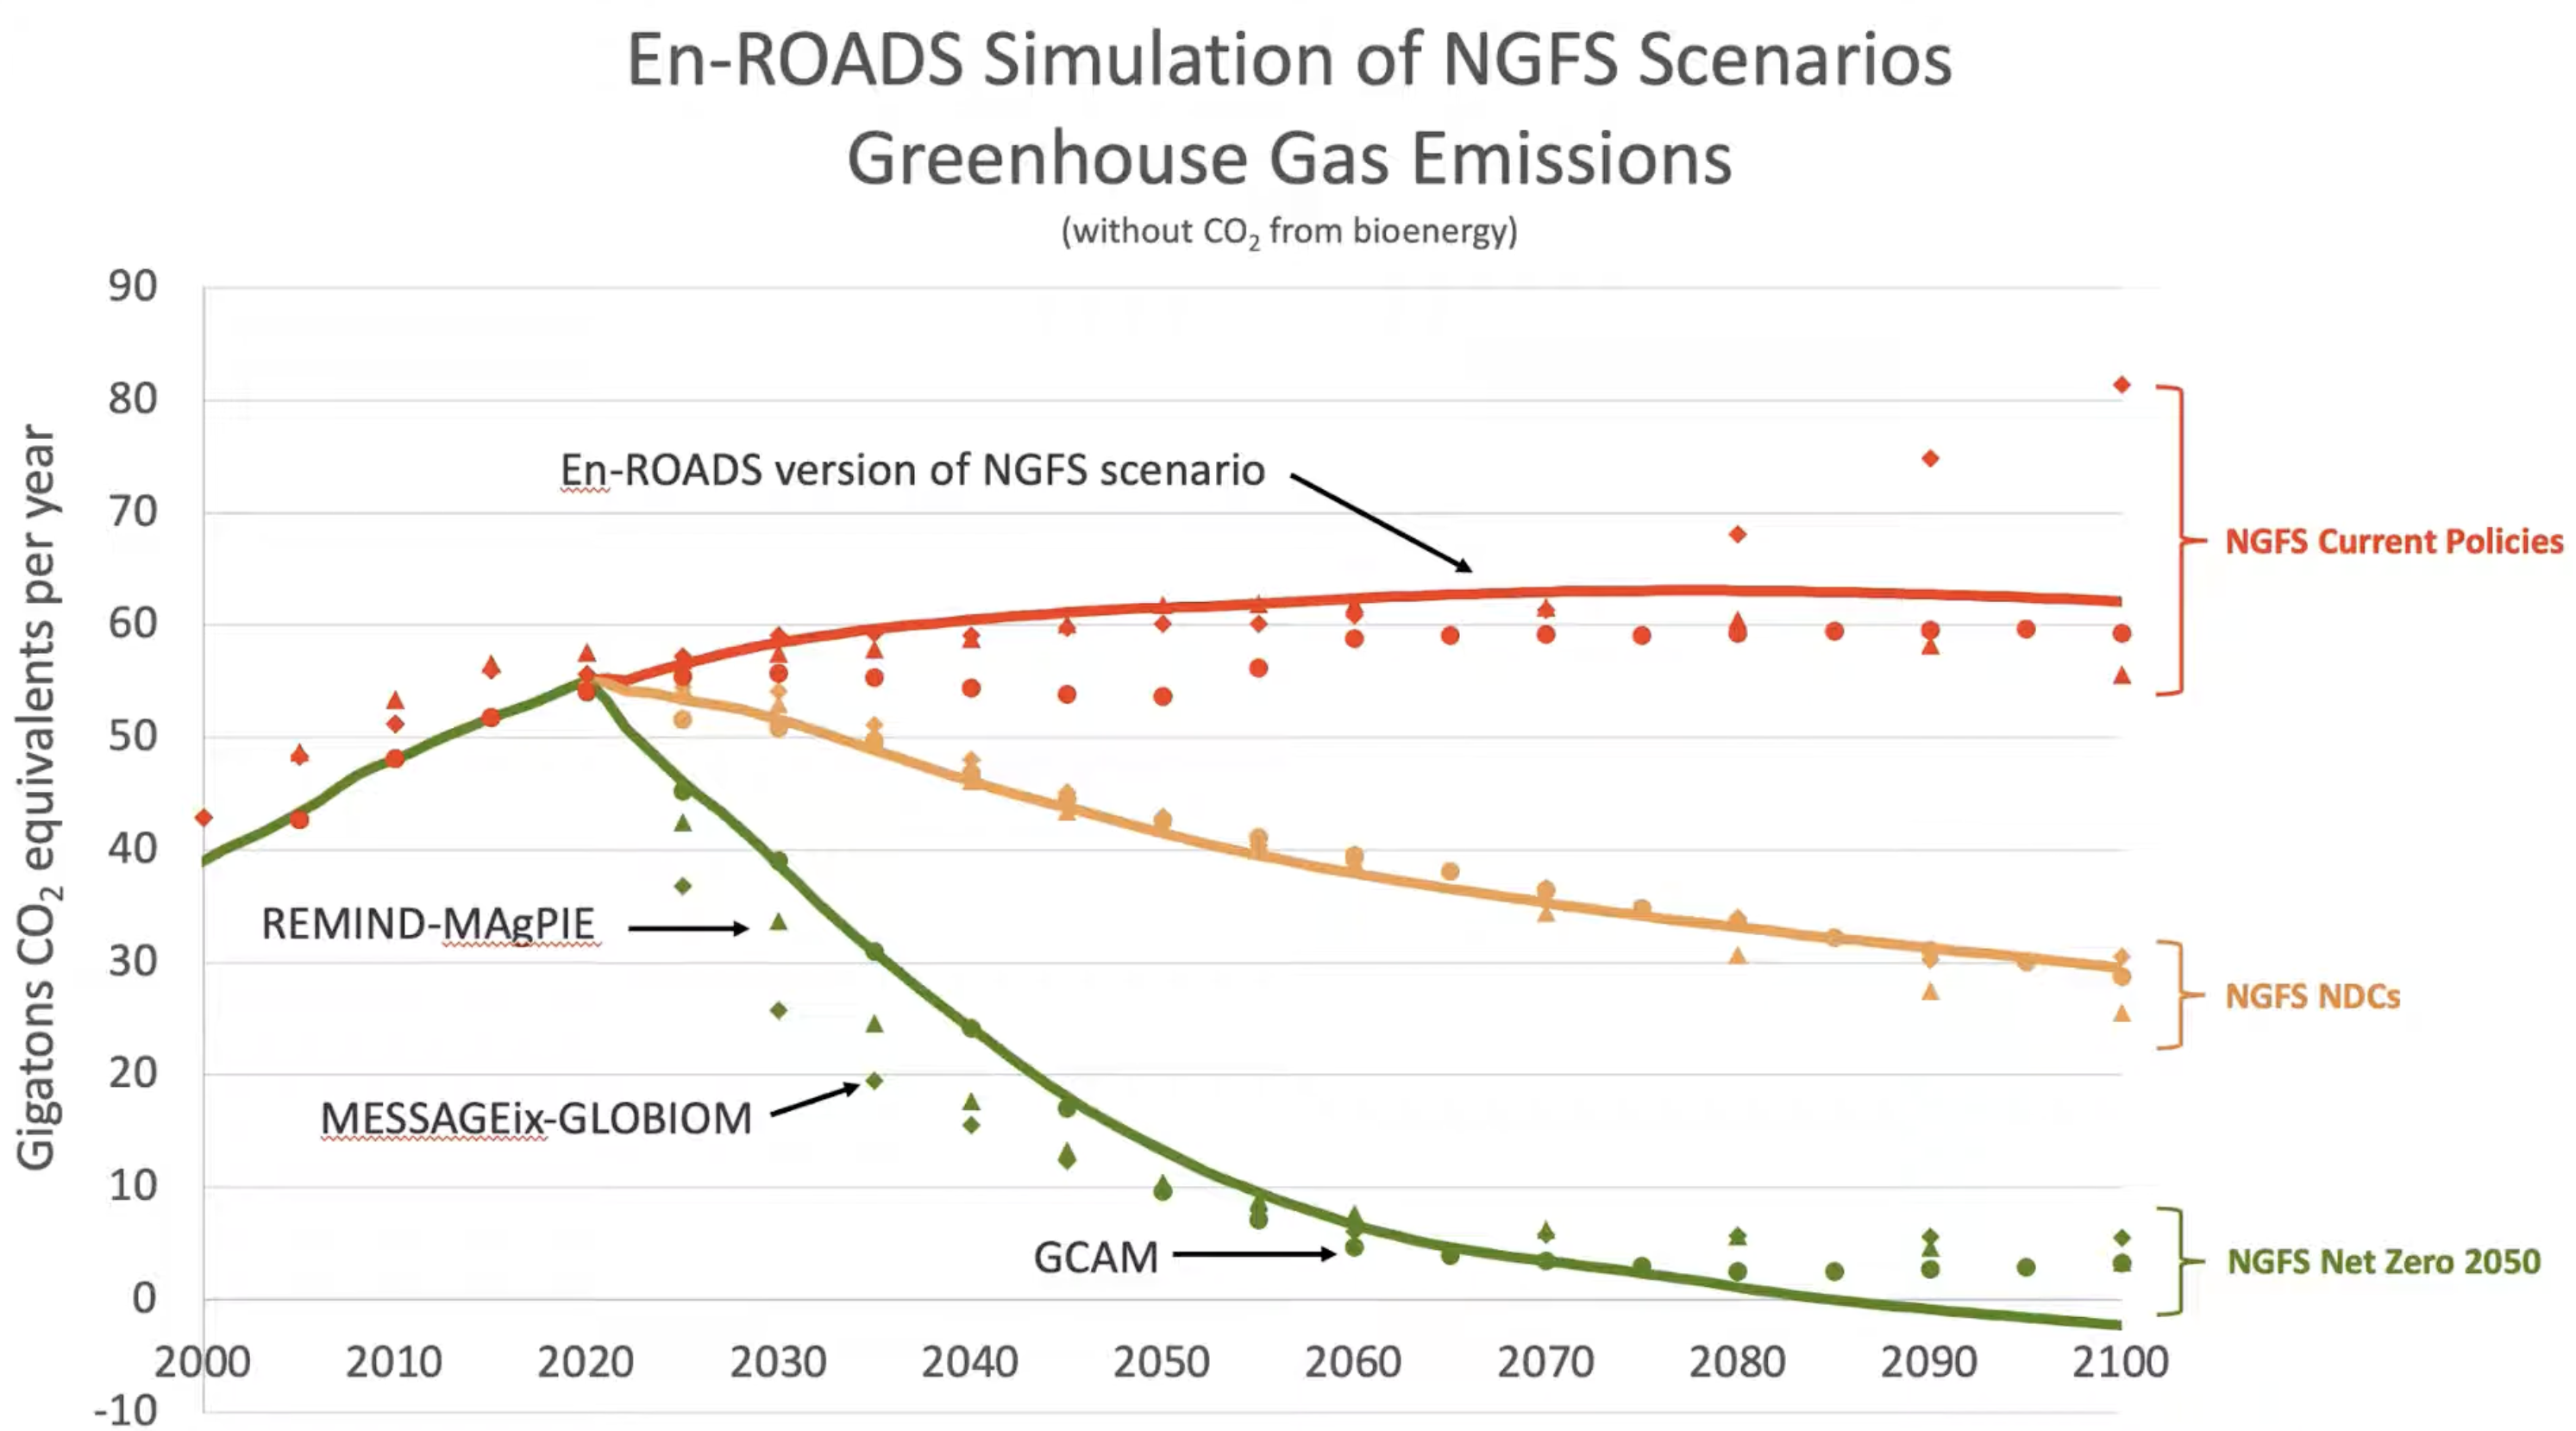
\includegraphics[width=\textwidth]{images/10_enroads-comparison-to-ngfs.png}

\newpage
%%%%%%%%%%%%%%%%%%%%%%%%%%%%%%%%%%%%%%%%%%%%%
\subsection{Identifying the climate science elements of the simulation}

In its default setup, the En-ROADS simulation shows a panel of two graphs and a temperature value (click the Home and reset icons to return to default).  Describe these three displays and explain their meanings.

\answerspace[7cm]

\noindent The primary outcome shown, {\em Greenhouse Gas Net Emissions}, is not a quantity we have explored before.  It would be useful to put it into context with other more familiar quanties (like atmospheric $\text{CO}_2$ concentrations and average temperature).  Using your own piece of graph paper, make a graph with {\em four} vertical axes (two on each side) showing these data sets\footnote{You should be able to find each of these datasets at \url{ourworldindata.com}, but access each individual plot {\bf by Googling} for, e.g., ``ourworldindata cumulative co2 emissions'' (the ourworldindata internal search engine is bad, so be sure to use google to access these plots).  Once at the data graph, remove all country data (``Clear'') and select only the ``World'' dataset; limit the time range using the slider.} --- Annual $\text{CO}_2$ emissions, Cumulative $\text{CO}_2$ emissions, Annual temperature anomaly, and atmospheric $\text{CO}_2$ (ppm) ---  and a horizontal axis showing time from 1975 to 2025.  \\[-6pt]

\noindent Examining your graphs, explain how our familiar quanties (atmospheric carbon dioxide and global temperature) relate to the emissions annual quantity plotted in En-ROADS.

\answerspace[5cm]

%%%%%%%%%%%%%%%%%%%%%
\newpage
\noindent Considering your own graphs, do you see any evidence for the statement\footnote{See, e.g., Figure 1b in Jeevanjee et al (AREPS 2025) and the related discussion.} that ``temperature is proportional to cumulative emissions''?

\answerspace[5cm]

\noindent What is the implication of this proporionality for the increase in temperature prior to a halt of $\text{CO}_2$ emissions, and the behavior of the temperature after the halt of $\text{CO}_2$ emissions?  Discuss this refererencing the figures shown below from Dessler Chapter 8.


\vfill

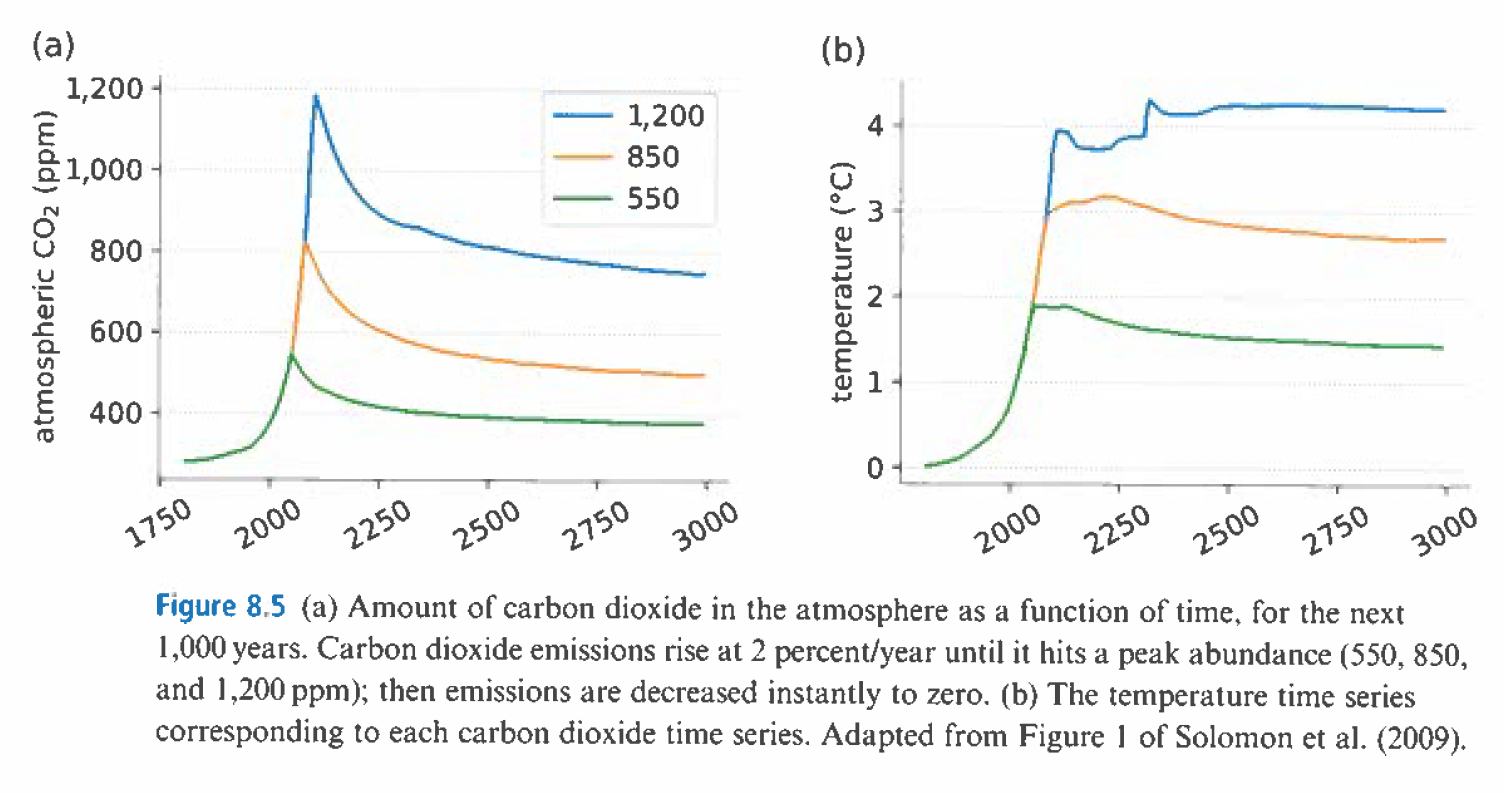
\includegraphics[width=\textwidth]{images/10_dessler_fig8-5.png}

%%%%%%%%%%%%%%%%%%%%%
\newpage

\noindent Returning to the simulation, let's examine the climate science inputs to the model and their effects on temperature.  There are three such parameters in the model, listed under {\em Simulation / Assumptions / Earth System / Climate System Sensitivities}.  List these quantities (one should be familiar to you, the other two we have not yet discussed) and define them based on information given at the model page and/or your own brief online research.  


\answerspace[7cm]

\noindent  Now use the {\em Assumptions} page to adjust these quantities and investigate their impact on the temperature graph.  Which has the most influence?  If we assume a $\pm 0.5\degree$C uncertainty in the ``Climate Sensitivity'', how much uncertainty does that lead to in the temperatures at 2050 and 2100?







 


\end{document}

